%%%%%%%%%%%%%%%%%%%%%%%%%%%%%%%%%%%%%%%%%
% Masters/Doctoral Thesis
% LaTeX Template
% Version 2.5 (27/8/17)
%
% This template was downloaded from:
% http://www.LaTeXTemplates.com
%
% Version 2.x major modifications by:
% Vel (vel@latextemplates.com)
%
% This template is based on a template by:
% Steve Gunn (http://users.ecs.soton.ac.uk/srg/softwaretools/document/templates/)
% Sunil Patel (http://www.sunilpatel.co.uk/thesis-template/)
%
% Template license:
% CC BY-NC-SA 3.0 (http://creativecommons.org/licenses/by-nc-sa/3.0/)
%
%%%%%%%%%%%%%%%%%%%%%%%%%%%%%%%%%%%%%%%%%

%------------------------------------------------------------------------------
% PACKAGES AND OTHER DOCUMENT CONFIGURATIONS
%------------------------------------------------------------------------------

\documentclass[
  11pt, % The default document font size, options: 10pt, 11pt, 12pt
  oneside, % Two side (alternating margins) for binding by default, uncomment to switch to one side
  ngerman, % ngerman for German
  singlespacing, % Single line spacing, alternatives: onehalfspacing or doublespacing
  %draft, % Uncomment to enable draft mode (no pictures, no links, overfull hboxes indicated)
  %nolistspacing, % If the document is onehalfspacing or doublespacing, uncomment this to set spacing in lists to single
  liststotoc, % Uncomment to add the list of figures/tables/etc to the table of contents
  %toctotoc, % Uncomment to add the main table of contents to the table of contents
  %parskip, % Uncomment to add space between paragraphs
  %nohyperref, % Uncomment to not load the hyperref package
  headsepline, % Uncomment to get a line under the header
  %chapterinoneline, % Uncomment to place the chapter title next to the number on one line
  %consistentlayout, % Uncomment to change the layout of the declaration, abstract and acknowledgements pages to match the default layout
]{MastersDoctoralThesis} % The class file specifying the document structure

\usepackage[utf8]{inputenc} % Required for inputting international characters
\usepackage[T1]{fontenc} % Output font encoding for international characters

\usepackage{mathpazo} % Use the Palatino font by default

\usepackage[backend=bibtex,style=authoryear,natbib=true]{biblatex} % Use the bibtex backend with the authoryear citation style (which resembles APA)

%\addbibresource{example.bib} % The filename of the bibliography

\usepackage[autostyle=true]{csquotes} % Required to generate language-dependent quotes in the bibliography

\usepackage{makecell}
\usepackage{listings}

% YML
\newcommand\YAMLcolonstyle{\color{red}\mdseries}
\newcommand\YAMLkeystyle{\color{black}\bfseries}
\newcommand\YAMLvaluestyle{\color{blue}\mdseries}
\makeatletter
\newcommand\language@yaml{yaml}
\expandafter\expandafter\expandafter\lstdefinelanguage
\expandafter{\language@yaml}
{
keywords={true,false,null,y,n},
keywordstyle=\color{darkgray}\bfseries,
basicstyle=\YAMLkeystyle,                                 % assuming a key comes first
sensitive=false,
comment=[l]{\#},
morecomment=[s]{/*}{*/},
commentstyle=\color{purple}\ttfamily,
stringstyle=\YAMLvaluestyle\ttfamily,
moredelim=[l][\color{orange}]{\&},
moredelim=[l][\color{magenta}]{*},
moredelim=**[il][\YAMLcolonstyle{:}\YAMLvaluestyle]{:},   % switch to value style at :
morestring=[b]',
morestring=[b]",
literate =    {---}{{\ProcessThreeDashes}}3
{>}{{\textcolor{red}\textgreater}}1
{|}{{\textcolor{red}\textbar}}1
{\ -\ }{{\mdseries\ -\ }}3,
}

% switch to key style at EOL
\lst@AddToHook{EveryLine}{\ifx\lst@language\language@yaml\YAMLkeystyle\fi}
\makeatother

\newcommand\ProcessThreeDashes{\llap{\color{cyan}\mdseries-{-}-}}

\definecolor{commentgreen}{RGB}{2,112,10}
\definecolor{eminence}{RGB}{108,48,130}
\definecolor{weborange}{RGB}{255,165,0}
\definecolor{frenchplum}{RGB}{129,20,83}

\lstdefinelanguage{elixir}{
  morekeywords={case,catch,def,do,else,false,%
      use,alias,receive,timeout,defmacro,defp,%
      for,if,import,defmodule,defprotocol,%
      nil,defmacrop,defoverridable,defimpl,%
      super,fn,raise,true,try,end,with,%
      unless},
  otherkeywords={<-,->, |>, \%\{, \}, \{, \, (, )},
  sensitive=true,
  morecomment=[l]{\#},
  morecomment=[n]{/*}{*/},
  morecomment=[s][\color{purple}]{:}{\ },
  morestring=[s][\color{orange}]"",
  morestring=[s][\color{orange}]'',
  commentstyle=\color{commentgreen},
  keywordstyle=\color{eminence},
  stringstyle=\color{red},
  basicstyle=\ttfamily,
  breaklines,
  showstringspaces=false,
  frame=tb
}

\lstset{numbers=left,xleftmargin=1em,frame=single,framexleftmargin=0em,numberstyle=\footnotesize\ttfamily}

%------------------------------------------------------------------------------
% MARGIN SETTINGS
%------------------------------------------------------------------------------

\geometry{
  paper=a4paper, % Change to letterpaper for US letter
  inner=2.5cm, % Inner margin
  outer=3.8cm, % Outer margin
  bindingoffset=.5cm, % Binding offset
  top=1.5cm, % Top margin
  bottom=1.5cm, % Bottom margin
  %showframe, % Uncomment to show how the type block is set on the page
}

\providecommand{\tightlist}{%
  \setlength{\itemsep}{0pt}\setlength{\parskip}{0pt}}

%------------------------------------------------------------------------------
% THESIS INFORMATION
%------------------------------------------------------------------------------

\thesistitle{Konzertkalender} % Your thesis title, this is used in the title and abstract, print it elsewhere with \ttitle
\supervisor{Sandro Bertolino} % Your supervisor's name, this is used in the title page, print it elsewhere with \supname
\examiner{} % Your examiner's name, this is not currently used anywhere in the template, print it elsewhere with \examname
\degree{Dipl. Techniker Informatik} % Your degree name, this is used in the title page and abstract, print it elsewhere with \degreename
\author{Damian Senn} % Your name, this is used in the title page and abstract, print it elsewhere with \authorname
\addresses{} % Your address, this is not currently used anywhere in the template, print it elsewhere with \addressname

\subject{} % Your subject area, this is not currently used anywhere in the template, print it elsewhere with \subjectname
\keywords{} % Keywords for your thesis, this is not currently used anywhere in the template, print it elsewhere with \keywordnames
\university{\href{http://www.tsbe.ch}{TSBE}} % Your university's name and URL, this is used in the title page and abstract, print it elsewhere with \univname
\department{} % Your department's name and URL, this is used in the title page and abstract, print it elsewhere with \deptname
\group{} % Your research group's name and URL, this is used in the title page, print it elsewhere with \groupname
\faculty{} % Your faculty's name and URL, this is used in the title page and abstract, print it elsewhere with \facname

\AtBeginDocument{
  \hypersetup{pdftitle=\ttitle} % Set the PDF's title to your title
  \hypersetup{pdfauthor=\authorname} % Set the PDF's author to your name
  \hypersetup{pdfkeywords=\keywordnames} % Set the PDF's keywords to your keywords
}

\begin{document}

\frontmatter % Use roman page numbering style (i, ii, iii, iv...) for the pre-content pages

\pagestyle{plain} % Default to the plain heading style until the thesis style is called for the body content

%------------------------------------------------------------------------------
% TITLE PAGE
%------------------------------------------------------------------------------

\includepdf[trim=10mm 0mm 0mm 0mm, clip]{titelblatt.pdf}
\begin{titlepage}
  \begin{center}

    \vspace*{.06\textheight}
    {\scshape\LARGE \univname\par}\vspace{1.5cm} % University name
    \textsc{\Large Diplomarbeit}\\[0.5cm] % Thesis type

    \HRule \\[0.4cm] % Horizontal line
    {\huge \bfseries \ttitle\par}\vspace{0.4cm} % Thesis title
    \HRule \\[1.5cm] % Horizontal line

    \begin{minipage}[t]{0.4\textwidth}
      \begin{flushleft} \large
        \emph{Author:}\\
        \href{mailto:damian.senn@gmail.com}{\authorname} % Author name - remove the \href bracket to remove the link
      \end{flushleft}
    \end{minipage}
    \begin{minipage}[t]{0.4\textwidth}
      \begin{flushright} \large
        \emph{Experten:} \\
        \href{mailto:sandro@bertolino.ch}{\supname}\\
        \href{mailto:raez@puzzle.ch}{Severin Räz}
      \end{flushright}
    \end{minipage}\\[3cm]

    \vfill

    \large \textit{Eine Diplomarbeit für den Abschluss \degreename}\\[0.3cm] % University requirement text

    \vfill

    {\large \today}\\[4cm] % Date
    %\includegraphics{Logo} % University/department logo - uncomment to place it

    \vfill
  \end{center}
\end{titlepage}

%------------------------------------------------------------------------------
% DECLARATION PAGE
%------------------------------------------------------------------------------

\begin{declaration}
  \addchaptertocentry{\authorshipname} % Add the declaration to the table of contents
  \noindent Mit meiner Unterschrift bestätige ich, die vorliegende Diplomarbeit
  selbstständig, ohne Hilfe Dritter und nur unter Benutzung der angegebenen
  Quellen ohne Copyright-Verletzung, erstellt zu haben.\\

  \noindent Unterschrift:\\
  \rule[0.5em]{25em}{0.5pt}

  \noindent Ort:\\
  \rule[0.5em]{25em}{0.5pt}

  \noindent Datum:\\
  \rule[0.5em]{25em}{0.5pt}
\end{declaration}

\cleardoublepage

%------------------------------------------------------------------------------
% ABSTRACT PAGE
%------------------------------------------------------------------------------

\renewcommand{\abstractname}{Management Summary}
\begin{abstract}
  \addchaptertocentry{\abstractname} % Add the abstract to the table of contents
  Inhalt für Management Summary folgt hier\ldots
\end{abstract}

%------------------------------------------------------------------------------
% ACKNOWLEDGEMENTS
%------------------------------------------------------------------------------

\begin{acknowledgements}
  \addchaptertocentry{\acknowledgementname} % Add the acknowledgements to the table of contents
  TODO
\end{acknowledgements}

%------------------------------------------------------------------------------
% LIST OF CONTENTS/FIGURES/TABLES PAGES
%------------------------------------------------------------------------------

\tableofcontents % Prints the main table of contents

\listoffigures % Prints the list of figures

\listoftables % Prints the list of tables

%------------------------------------------------------------------------------
% ABBREVIATIONS
%------------------------------------------------------------------------------

\begin{abbreviations}{ll}

  \textbf{TSBE} & \textbf{T}elematik\textbf{s}chule \textbf{Be}rn\\
  \textbf{HTML} & \textbf{H}yper\textbf{t}ext \textbf{M}arkup \textbf{L}anguage\label{HTML}\\
  \textbf{CSS} & \textbf{C}ascading \textbf{S}yle \textbf{S}heets\label{CSS}\\
  \textbf{SASS} & \textbf{S}yntactically \textbf{A}wesome \textbf{S}tyle\textbf{s}heets\\
  \textbf{HTTP} & \textbf{H}yper\textbf{t}ext \textbf{T}ransfer \textbf{P}rotocol\\
  \textbf{SEO} & \textbf{S}earch \textbf{E}ngine \textbf{O}ptimization\label{SEO}\\
  \textbf{OWASP} & \textbf{O}pen \textbf{W}eb \textbf{A}pplication \textbf{S}ecurity \textbf{P}roject\label{OWASP}\\
  \textbf{XSS} & \textbf{Cross}-\textbf{s}ite \textbf{s}cripting\label{XSS}\\
  \textbf{SSR} & \textbf{S}erver \textbf{S}ide \textbf{R}endered\label{SSR}\\
  \textbf{CPC} & \textbf{C}ost \textbf{P}er \textbf{C}lick\\
  \textbf{CPM} & \textbf{C}ost \textbf{P}er \textbf{M}ile\\
  \textbf{SMTP} & \textbf{S}imple \textbf{M}ail \textbf{T}ransfer \textbf{P}rotocol\\
  \textbf{ERD} & \textbf{E}ntity \textbf{R}elationship \textbf{D}iagram\\
  \textbf{API} & \textbf{A}pplication \textbf{P}rogramming \textbf{I}nterface\\
  \textbf{JSON} & \textbf{J}ava\textbf{S}cript \textbf{O}bject \textbf{N}otation\\
  \textbf{URL} & \textbf{U}nified \textbf{R}esource \textbf{L}ocator\\
  \textbf{AWS} & \textbf{A}mazon \textbf{W}eb \textbf{S}ervices\\
  \textbf{SQL} & \textbf{S}tructured \textbf{Q}uery \textbf{L}anguage\\
  \textbf{NPM} & \textbf{N}ode \textbf{P}ackage \textbf{M}anager\\
  \textbf{OTP} & \textbf{O}pen \textbf{T}elecom \textbf{P}latform\\

\end{abbreviations}

%------------------------------------------------------------------------------
% DEDICATION
%------------------------------------------------------------------------------

\dedicatory{For/Dedicated to/To my\ldots}

%------------------------------------------------------------------------------
% CHAPTERS
%------------------------------------------------------------------------------

\mainmatter % Begin numeric (1,2,3...) page numbering

\pagestyle{thesis} % Return the page headers back to the "thesis" style

% Include the chapters of the thesis as separate files from the Chapters folder
% Uncomment the lines as you write the chapters

\chapter{Initialisierung}

\label{ReportInitialisierung}

\section{Ausgangslage}

Als regelmässiger Konzertbesucher wünsche ich mir eine Plattform im
Internet, auf welcher ich eine zuverlässige Übersicht an Konzerten in
meiner Umgebung vorfinde. Heute sind die Events nur verteilt auf
verschiedenen Seiten wie die der Venues, des Konzertveranstalters, des
Künstlers oder auf Facebook publiziert.\\

\noindent
Ich möchte deshalb eine zentrale Plattform entwickeln, die es Benutzern
einfach macht, Konzerte für ihren Geschmack zu finden.
Die Plattform soll Genre unabhängig sein und entsprechende Filter anbieten.
Den Benutzern der Plattform soll es möglich sein, Konzerte selber zu
erfassen und pflegen.\\

\noindent
Um einen zusätzlichen Service für den Benutzer zur Verfügungs zu stellen,
ist es auch denkbar, eine Art Notifikationssystem zu bauen um Benutzer
über Handy-Notifications oder per Email an Konzerte oder Künstler zu
erinnern.\\

\noindent
Konzertveranstaltern kann das Erfassen ihrer Events vereinfacht werden,
indem auf der Plattform erfasste Veranstaltungen direkt auf den Sozialen
Medien wie Facebook, Twitter oder Instagram geteilt werden können.


\clearpage
\section{Projektziele}

Folgende Ziele sind in der Initialisierungsphase definiert worden:

\begin{longtable}[]{@{}llc@{}}
  \toprule
  Nr.  & Zielbeschreibung                                                                       & Muss/Kann\tabularnewline
  \toprule
       & Produktziele\tabularnewline
  \midrule
  1.1  & Besucher können im Produkt nach Konzerten suchen                                       & \textbf{Muss}\tabularnewline
  1.2  & Suchresultate können nach Musik-Genre und Ort gefiltert werden                         & \textbf{Muss}\tabularnewline
  1.3  & Das Produkt soll ein modernes responsives Design vorweisen                             & \textbf{Muss}\tabularnewline
  1.4  & Konzerte sollen von Suchmaschinen indexiert werden können                              & \textbf{Muss}\tabularnewline
  1.5  & Benutzer können isch im Produkt registrieren                                           & \textbf{Muss}\tabularnewline
  1.6  & Benutzer können ihr Passwort nach Verlust neu setzen                                   & \textbf{Muss}\tabularnewline
  1.7  & Inhalte des Portals sind durch die Benutzer erfassbar und bearbeitbar                  & \textbf{Muss}\tabularnewline
  1.8  & Kompatibilität mit aktuellem Google Chrome und Mozilla Firefox Browser                 & \textbf{Muss}\tabularnewline
  1.9  & Konzerte können vom Produkt nach Facebook exportiert werden                            & Kann\tabularnewline
  1.10 & Ein angemeldeter Benutzer kann vermerken ob er einem Konzert teilnimmt                 & Kann\tabularnewline
  1.11 & Das Produkt soll sich an Security Best-Practices von OWASP halten                      & \textbf{Muss}\tabularnewline
  \bottomrule
       & Abwicklungsziele\tabularnewline
  \midrule
  2.1  & \makecell[l]{Das Projekt soll nach HERMES 5 unter Berücksichtigung der Richtlinien von                                \\ der TSBE dokumentiert werden} & \textbf{Muss}\tabularnewline
  2.2  & Das Produkt muss bis Projektende fertiggestellt und bereit für die Einführung sein     & \textbf{Muss}\tabularnewline
  2.3  & Die Technische-Umsetzung wird durch Damian Senn erstellt                               & \textbf{Muss}\tabularnewline
  2.4  & \makecell[l]{Die Kommunikation zwischen Experten und Diplomanden erfolgt wie im                                       \\ Projektauftrag \ref{kommunikation} beschrieben.} & \textbf{Muss}\tabularnewline
  2.5  & Das Projekt muss bis Ende Mai 2019 abgeschlossen sein                                  & \textbf{Muss}\tabularnewline
  \bottomrule
\end{longtable}


\clearpage

\section{Projektorganisation}

\begin{figure}[!htb]
  \centering
  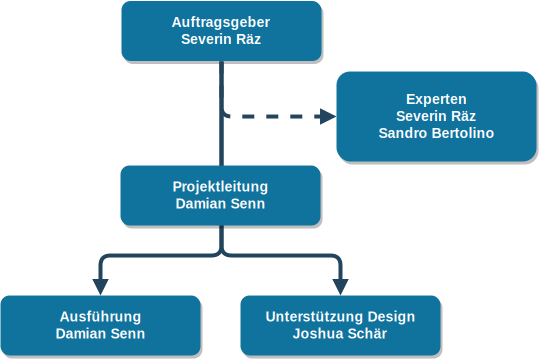
\includegraphics[width=0.8\textwidth]{figures/organigram.png}
  \caption{Organigram}
\end{figure}

\includepdf[pagecommand={\section{Ausgefüllter Projektplan}}]{figures/planung-final.pdf}

\section{Lieferergebnisse}

\begin{itemize}
  \tightlist{}
  \item{}Studie (Anhang~\ref{AppendixStudie})
  \item{}Projektauftrag (Anhang~\ref{AppendixProjektauftrag})
  \item{}Konzept (Anhang~\ref{AppendixKonzept})
\end{itemize}

\section{Ressourcenplan}

\section{Risiken}

\clearpage

\section{Abgrenzungen}

\begin{figure}[!htb]
  \centering
  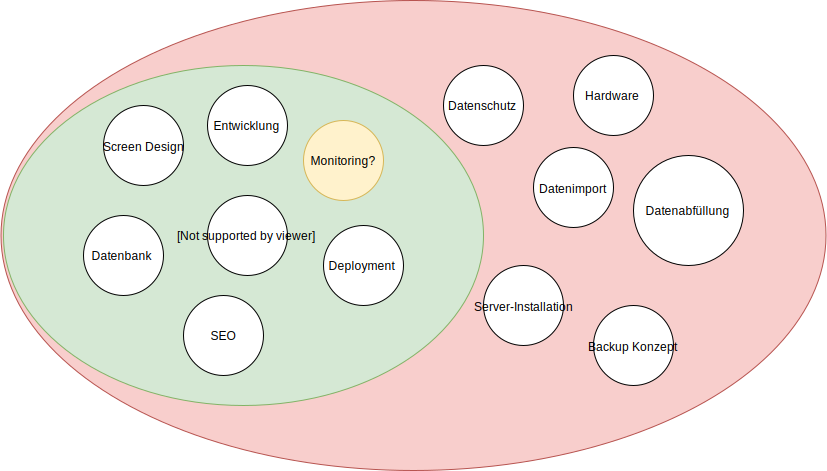
\includegraphics[width=0.95\textwidth]{figures/abgrenzungen.png}
  \caption{Abgrenzungen}
\end{figure}

Die detaillierten Erklärung zu den Abgrenzungen sind im Projektauftrag~\ref{abgrenzungen} zu finden.

\clearpage

\section{Studie}

\subsection{Informationsbeschaffung}

Folgende Quellen wurden in diesem Projekt für die Informationsbeschaffung
genutzt:

\begin{longtable}[]{@{}p{3cm}p{10cm}@{}}
  \toprule
  \textbf{Quelle}               & \textbf{Beschreibung}\tabularnewline
  \toprule
  Schulwissen / Berufserfahrung & Die Grundlage für die Umsetzung dieses Projekts wird durch mein existierendes Schulwissen sowie meine langjährige Berufserfahrung in der Software-Entwicklung gesetzt.\tabularnewline
  \midrule
  Internet                      & Ein Grossteil der Informationen werden heute über das Internet bezogen, für die Evaluation von Technologien und Lösungsansätzen wird einiges über das Internet recherchiert werden müssen.\tabularnewline
  \midrule
  Externer Experte              & Bei konzeptionellen sowie technischen Fragen kann der externe Experte um Rat gefragt werden.\tabularnewline
  \bottomrule
  \caption{Informationsbeschaffung}
\end{longtable}


\clearpage
\subsection{Anforderungskatalog}

Im Anforderungskatalog werden die Muss- und Kann-Kriterien definiert.
Muss-Kriterien sind zwingend zu erfüllen, Kann-Kriterien sind als optionale
Erweiterung zu verstehen.

% TODO: Fix multirows across pages
%       https://tex.stackexchange.com/questions/79143/how-to-repeat-cell-content-on-next-page-for-longtable-using-multirow/79152
\begin{longtable}[]{@{}p{1.9cm}p{2.5cm}cp{5.5cm}cc@{}}
  \toprule
  \textbf{Feature}                & \textbf{Titel}             & \textbf{Nr.} & \textbf{Kriterium}                                                                                          & \textbf{Ziel} & \textbf{Muss}\tabularnewline
  \midrule
  \endhead
  \multirow{10}{*}{Suche}         & Suche nach Konzertname     & 1.1          & Listet alle Konzerte die Wörter der Suche im Konzertnamen beinhalten                                        & 1.1           & \textbf{Muss}                \\ \cline{2-6}
                                  & Suche nach Konzertlocation & 1.2          & Schränkt die Such-Resultate nach gegebener Konzertlocation ein                                              & 1.2           & \textbf{Muss}                \\ \cline{2-6}
                                  & Suche nach Ort             & 1.2          & Schränkt die Such-Resultate nach gegebenem Ort ein                                                          & 1.2           & \textbf{Muss}                \\ \cline{2-6}
                                  & Suche nach Genre           & 1.2          & Schränkt die Such-Resultate nach gegebenem Musik-Genre ein                                                  & 1.2           & \textbf{Muss}                \\
  \midrule
  \multirow{8}{*}{Design}         & Desktop                    & 2.1          & Alle Ansichten haben eine Desktop-Optimierte Variante                                                       & 1.4           & \textbf{Muss}                \\ \cline{2-6}
                                  & Tablet                     & 2.2          & Alle Ansichten haben eine Tablet-Optimierte Variante                                                        & 1.4           & \textbf{Muss}                \\ \cline{2-6}
                                  & Mobile                     & 2.3          & Alle Ansichten haben eine Mobile-Optimierte Variante                                                        & 1.4           & \textbf{Muss}                \\ \cline{2-6}
                                  & Browser Kompatibilität     & 2.4          & Alle Ansichten müssen in aktuellem Google Chrome und Mozilla Firefox dem Grundlayout folgen                 & 1.9           & \textbf{Muss}                \\
  \midrule
  \multirow{4}{*}{\acrshort{seo}} & Indexierbarkeit            & 3.1          & Das Produkt ist von Suchmaschinen indexierbar                                                               & 1.5           & \textbf{Muss}                \\ \cline{2-6}
                                  & Linked Data                & 3.2          & Konzert Detailseiten sind mit dem Event-Schema\footnote{\url{https://schema.org/MusicEvent}} ausgestattet   & 1.5           & \textbf{Muss}                \\
  \midrule
  \multirow{8}{*}{Benutzer}       & Registrierung              & 4.1          & Besucher können sich einen Benutzer registrieren, Benutzernamen und E-Mail Adressen müssen einzigartig sein & 1.6           & \textbf{Muss}                \\ \cline{2-6}
                                  & Passwort-Vergessen         & 4.2          & Benutzer können sich einen Passwort-Reset Link anfordern                                                    & 1.7           & \textbf{Muss}                \\ \cline{2-6}
                                  & Social                     & 4.3          & Benutzer können auf Konzerten vermerken ob sie Teilnehmen oder nicht                                        & 1.11          & Kann                         \\
  \midrule
  \clearpage
  \multirow{6}{*}{Erfassung}      & Artist                     & 5.1          & Benutzer können Artisten mit einem Genre erfassen                                                           & 1.8           & \textbf{Muss}                \\ \cline{2-6}
                                  & Location                   & 5.2          & Benutzer können eine Konzertlocation mit Ort/Strasse erfassen                                               & 1.8           & \textbf{Muss}                \\ \cline{2-6}
                                  & Konzert                    & 5.3          & Benutzer können ein Konzert mit Konzertlocation und Artisten erfassen                                       & 1.8           & \textbf{Muss}                \\ \cline{2-6}
                                  & Facebook                   & 5.4          & Benutzer können ein Konzert in ein Facebook-Event exportieren                                               & 1.10          & Kann                         \\
  \midrule
  \multirow{9}{*}{Security}       & SQL-Injection              & 6.1          & Das Produkt soll resistent gegen SQL-Injection sein                                                         & 1.12          & \textbf{Muss}                \\ \cline{2-6}
                                  & HTML-Injection             & 6.2          & Das Produkt soll resistent gegen HTML-Injection / \acrshort{xss} sein                                       & 1.12          & \textbf{Muss}                \\ \cline{2-6}
                                  & Passwort encryption        & 6.3          & Passwörter von Benutzer müssen mit einem sicheren Verfahren gespeichert werden                              & 1.12          & \textbf{Muss}                \\ \cline{2-6}
                                  & Session                    & 6.4          & Session-Cookies dürfen nicht durch JavaScript ausgelesen werden                                             & 1.12          & Kann                         \\
  \midrule
  Performance                     & Ladezeit                   & 7.1          & Die Seitenansichten dürfen nicht länger als 6 Sekunden auf einem 3G Netz laden                              &               & \textbf{Muss}                \\
  \midrule
  Sonstiges                       & User Tracking              & 8.1          & Benutzerverhalten soll analysiert und nachvollziehbar sein.                                                 &               & Kann                         \\
  \bottomrule
  \caption{Anforderungskatalog}
\end{longtable}


\subsection{Mögliche Varianten}

\subsection{Evaluation Varianten}

\subsection{Entscheid Varianten}

\clearpage
\section{Wirtschaftlichkeit}

\subsection{Projektkosten}

Für die Berechnung der Projektkosten wird ein Stundensatz von 150.- CHF angenommen.

\begin{longtable}[]{@{}lrr@{}}
  \toprule
  \textbf{Phase}  & \makecell[r]{\textbf{Geplante}                               \\\textbf{Stunden}} & \textbf{Kosten}\tabularnewline
  \midrule
  \endhead
  Initialisierung & 64                             & 9'600.- CHF\tabularnewline
  Konzept         & 66                             & 9'900.- CHF\tabularnewline
  Realisierung    & 136                            & 20'400.- CHF\tabularnewline
  Abschluss       & 36                             & 5'400.- CHF\tabularnewline
  \midrule
  \textbf{Total:} & 286                            & 42'900.- CHF\tabularnewline
  \bottomrule
  \caption{Projektkosten}
\end{longtable}


\noindent
Die geplanten Projektkosten betragen somit \textbf{42'900.- CHF}.

\begin{longtable}[]{@{}lll@{}}
  \toprule
  \textbf{Kostenstelle} & \textbf{Jährliche Kosten}\tabularnewline
  \midrule
  \endhead
  Software              & Keine\tabularnewline
  .com Domain           & 20.- CHF\tabularnewline
  Hosting               & 1'800.- CHF\tabularnewline
  \midrule
  \textbf{Total:}       & 1'820.- CHF\tabularnewline
  \bottomrule
  \caption{Betriebskosten}
\end{longtable}


Für die Betriebskosten eines Hostings wird einen durchschnittlichen monatlichen
Preis von 150.- CHF angenommen, da das Deployment für dieses nicht vorgesehen
ist, ist dies eine von Damian Senn geschätzte Zahl.

\clearpage
\subsection{Break Even Analyse}\label{break-even-analyse}

\subsubsection{Gigboost}

Beim Modell «Gigboost» wird Benutzern eine Option angeboten bei der ihre
publizierten Gigs auf der Startseite sowie in Suchresultaten anderen Einträgen
bevorzugt dargestellt werden. Für einen Gegenpreis von 10.- CHF kann ein Benutzer
seinen Gig «boosten».

\begin{figure}[!htb]
  \centering
  \includegraphics[width=0.95\textwidth]{initialisierung/wirtschaftlichkeit-gigboost.png}
  \caption{Break-Even Analyse - Gigboost}
\end{figure}

\clearpage
\subsubsection{Werbung}\label{break-even-analyse-werbung}

Im Modell «Werbung» wird ausgerechnet wieviele aktive Benutzer das Produkt benötigt
um in den nächsten Jahren Gewinn zu erzielen.

Durch Annahme von einem Erlös von \textbf{140.- CHF} pro \textbf{40'0000 Besucher}\footnote{\url{https://www.quora.com/How-much-does-Google-AdSense-pay-for-3-banners-on-a-webpage-per-1-000-views/answer/Manas-Sahu-59}} erhalten wir folgendes Bild:

\begin{figure}[!htb]
  \centering
  \includegraphics[width=0.95\textwidth]{initialisierung/wirtschaftlichkeit-werbung.png}
  \caption{Break-Even Analyse - Werbung}
\end{figure}

\begin{longtable}[]{@{}lll@{}}
  \toprule
  \textbf{Besucher pro Tag} & \textbf{Erlös pro Tag} & \textbf{Erlös pro Monat}\tabularnewline
  2'000                     & 7.- CHF                & 210.- CHF\tabularnewline
  4'000                     & 14.- CHF               & 420.- CHF\tabularnewline
  8'000                     & 28.- CHF               & 840.- CHF\tabularnewline
  12'000                    & 42.- CHF               & 1'260.- CHF\tabularnewline
  16'000                    & 46.- CHF               & 1'680.- CHF\tabularnewline
  \bottomrule
  \caption{Werbeeinnahmen pro Besucher}
\end{longtable}

Der Grafik ist zu entnehmen, dass das Produkt bei 8'000 Besucher pro Tag nach ca. 6 Jahren Gewinn erzielt. Bei 12'000 Besucher pro Tag erzielt das Produkt nach bereits 4 Jahren Gewinn und mit 16'000 Beucher pro Tag schon im dritten Jahr.


\chapter{Konzept}

\label{AppendixKonzept}

\section{Zweck des Dokuments}\label{KonzeptZweck}

Das Konzept dient als Anleitung für die Realisierungsphase. Die in der Konzept
erarbeiteten Details müssen in der Realisierung eingehalten un umgesetzt
werden.

\subsection{Teilkonzepte}

Durch die in der Studie gewonnenen Erkentnissen, werden in der Phase Konzept
verschiedene Teilkonzepte erstellt.

Im Teilkonzept «Portalname» wird der Name des Produktes erarbeitet.

Im Teilkonzept «Design- und Bedienkonzept» werden die Ansichten der Applikation
in Mockups umgesetzt. Es werden die Benutzer Use-Cases vom Besucher sowie der
Konzert-Erfasser aufgezeigt.

Im Teilkonzept «Softwarekonzept» werden die Datenflüsse hinter den Mockups
aufgezeigt, sowie die Datenbankstruktur aufgebaut.

Im Teilkonzept «Testkonzept» werden die einzelnen Systemtests aufgelistet sowie
ausgearbeitet wie granular welche Teile der Software getestet werden sollen.

Im letzten Teil des Konzept-Dokuments wird im Fazit dokumentiert, wie und warum
das Konzept von den vorhergehenden Phasen des Projekts abweicht.


\clearpage
\section{Portalname}\label{portalname}

Der Portalname wurde in einer Brainstorming-Session von Damian Senn auf
den Namen \textbf{«Gigpillar»} festgelegt. Der Name ist angelehnt an die Werbepfeiler in
Städten, wo oft Werbeplakate für Konzerte hängen.

Die folgenden Ideen wurden in Betracht gezogen, jedoch war keine Domain mehr
verfügbar oder der Name überzeugte nicht:

\begin{itemize}
  \item{} upto.com («What are you up to?»)
  \item{} up-to.com
  \item{} uptoin.com
  \item{} gigup.com
  \item{} gigsta.com («Gigs to attend»)
  \item{} gigin.com
  \item{} gigsin.com
  \item{} gixin.com («Gigs in»)
  \item{} dualact.com («Loud act»)
  \item{} trecnoc.com («Concert» rückwärts)
\end{itemize}

\clearpage
\section{Design- und Bedienkonzept}\label{design--und-bedienkonzept}

\subsection{Mockups}

\subsubsection{Homepage}

Die Homepage ist die erste Seite, die der Besucher sieht, wenn er/sie die
Applikation direkt über \href{https://gigpillar.com/}{gigpillar.com} aufruft.
Auf den ersten Blick ist die Suche sowie ein grosses Bild (Banner) eines Gigs
zu erblicken. Weiter sind Links zu gängigen Funktionalitäten wie Gig hinzufügen
sowie das Login in einer Navigation erreichbar.

Unter dem Banner werden Gigs in nächster nähe des Besuchers aufgelistet, der
Link «change location» führt weiter zur Suchresultate Seite um den
entsprechenden Filter anzupassen.

\begin{figure}[!htb]
  \centering
  \includegraphics[width=0.95\textwidth]{mockups/homepage.png}
  \caption{Mockup: Homepage}
\end{figure}

\clearpage
\subsubsection{Suchresultate}

Auf der Suchresultate Seite sieht der Benutzer seine Suchresultate der von der
globalen Suchbox ausgelösten Suche. Die Seite bietet weitere Filter an um die
Resultate weiter einzugrenzen.\\

\noindent
Folgende Filter stehen den Benutzern zur Verfügung:

% TODO: This diverges from our search criteria described in the previous phase.

\begin{itemize}
  \tightlist{}
  \item{} Ort
  \item{} Datum von
  \item{} Datum bis
  \item{} Musik Genre
\end{itemize}

\noindent
Das Anwählen eines Suchresultates führt den Benutzer weiter zur detaillierten
Gig Ansicht.

\begin{figure}[!htb]
  \centering
  \includegraphics[width=0.95\textwidth]{mockups/search-result.png}
  \caption{Mockup: Suchresultate}
\end{figure}

\clearpage
\subsubsection{Gig Ansicht}

In der Gig Ansicht werden alle Details zu einem Event aufgelistet.

\begin{itemize}
  \tightlist{}
  \item{} Datum des Events
  \item{} Zeit wann das Event beginnt, bzw die Location die Türen öffnet
  \item{} Liste aller Künstler mit optionaler Startzeit
  \item{} Eine Beschreibung des Events
  \item{} Die Adresse der Location mit Link auf Google Maps
\end{itemize}

\noindent
Ausserdem soll es den Benutzern möglich sein, über einen «Add to my calendar»
Link das Event zu seiner Kalender-Applikation zu importieren.

\begin{figure}[!htb]
  \centering
  \includegraphics[width=0.95\textwidth]{mockups/event.png}
  \caption{Mockup: Gig Ansicht}
\end{figure}

\clearpage
\subsubsection{Gig erfassen}

Benutzer können Gigs erfassen.\\

\noindent
Folgende Daten sind für einen Gig zu erfassen:

\begin{itemize}
  \tightlist{}
  \item{} Name
  \item{} Bild \textit{(optional)}
  \item{} Location
  \item{} Datum
  \item{} Zeit
  \item{} Eine Liste von Artists mit optionaler Startzeit
  \item{} Beschreibung
  \item{} Link zum Ticketvertreiber
\end{itemize}

\begin{figure}[!htb]
  \centering
  \includegraphics[width=0.95\textwidth]{mockups/add-gig.png}
  \caption{Mockup: Gig erfassen}
\end{figure}

\clearpage
\subsubsection{Benutzerprofil}

Benutzer können ihr eigenes Profil verwalten und folgende Tätigkeiten
verrichten:

\begin{itemize}
  \tightlist{}
  \item{} Anzeigename ändern
  \item{} E-Mail Adresse ändern \textit{(mit E-Mail Bestätigung)}
  \item{} Passwort ändern \textit{(muss vorher altes Passwort bestätigen)}
  \item{} Account löschen \textit{(muss doppelt bestätigt werden!)}
\end{itemize}

\begin{figure}[!htb]
  \centering
  \includegraphics[width=0.95\textwidth]{mockups/profile.png}
  \caption{Mockup: Benutzerprofil}
\end{figure}

\clearpage
\subsection{Genre Filter}\label{genrefilter}

Der Genre Filter soll folgende Werte zur Verfügung stellen.

\begin{itemize}
  \item{} Alternative
  \item{} Blues
  \item{} Classical
  \item{} EDM
  \item{} Hip-Hop
  \item{} Jazz
  \item{} Metal
  \item{} Pop
  \item{} Punk
  \item{} Reggae
  \item{} Rock
\end{itemize}

\clearpage
\section{Softwarekonzept}\label{softwarekonzept}
\subsection{Datenfluss}\label{datenfluss}

\subsubsection{Homepage}\label{datenfluss-homepage}

Die Homepage zeigt den Besuchern Gigs in ihrer Nähe an, dazu muss über eine
GeoIP API die IP-Adresse des Besuchers auf ein Land zurückverfolgt werden.
Dazu wird beim ersten Besuch die GeoIP API abgefragt und das Land des Benutzers
in eine Session geschrieben. Bei weiteren Aufrufen wird das Land direkt aus der
Session bezogen.

%GigPillarWeb
%GigPillarWeb_Session
%GigPillar
%GeoIp
%
%Response = GigPillarWeb./ {
%  if (hasSession) {
%    location = GigPillarWeb_Session.getLocation()
%  } else {
%    location = GigPillarWeb_Session.createSession() {
%      location = GeoIp.getLocation(ip)
%    }
%  }
%
%  Events = GigPillar.getUpcomingEvents(location)
%}

\begin{figure}[!htb]
  \centering
  \includegraphics[width=0.95\textwidth]{konzept/datenfluss-homepage.png}
  \caption{Datenfluss: Homepage}
\end{figure}

\clearpage
\subsubsection{Suchfeld}\label{datenfluss-suchfeld}

Das globale Suchfeld hat eine Autocompletion, welche Daten direkt von
der GigPillar Applikation bezieht. Die Daten für Städtenamen wird jedoch von
einer externen Datenquelle, z.B. Google Maps, bezogen.

%GigPillarWeb
%GigPillar
%GoogleMaps
%
%Response = GigPillarWeb./searchCompletion {
%  Cities = GoogleMaps.searchCities(searchParameters)
%  Locations = GigPillar.searchLocations(searchParameters)
%  Genres = GigPillar.searchGenres(searchParameters)
%  Artists = GigPillar.searchArtists(searchParameters)
%  Events = GigPillar.searchEvents(searchParameters)
%}

\begin{figure}[!htb]
  \centering
  \includegraphics[width=0.95\textwidth]{konzept/datenfluss-suchfeld.png}
  \caption{Datenfluss: Suchfeld}
\end{figure}

\clearpage
\subsubsection{Gig erstellen - Locationfeld}\label{datenfluss-gig-erstellen-locationfeld}

Beim Erstellen eines neuen Gigs, muss eine Location zugewiesen werden. Die
Locations werden über die bereits in GigPillar erfassten Locations sowie über
eine externe Datenquelle, wie z.B. Google Maps, bezogen.

%GigPillarWeb
%GigPillar
%GoogleMaps
%
%Response = GigPillarWeb./locationCompletion {
%  Locations = GigPillar.searchLocations(searchParameters) {
%    Locations = searchLocations(searchParameters)
%    Locations = GoogleMaps.searchLocations(searchParameters)
%  }
%}

\begin{figure}[!htb]
  \centering
  \includegraphics[width=0.95\textwidth]{konzept/datenfluss-locationfeld.png}
  \caption{Datenfluss: Gig erstellen - Locationfeld}
\end{figure}

%TODO:
%\clearpage
%\subsubsection{Gig erstellen - Artistfeld}

% Autocomplete, +lastfm?

%TODO:
%\clearpage
%\subsubsection{Gig erstellen}\label{datenfluss-gigerstellen}

% Optional FB-Event erstellen

\clearpage
\subsubsection{Passwort-Reset}\label{datenfluss-passwort-reset}

Falls ein Benutzer sein Passwort vergessen hat, kann dieser ein neues Passwort
über die Passwort-Reset Funktion setzen. Beim Auslösen eines Passwort-Resets,
wird dem Benutzer ein E-Mail mit einem Link zugeschickt.
Der Passwort-Reset-Link führt den Benutzer auf ein Formular auf welchem er/sie
die Möglichkeit hat, ein neues Passwort zu setzen.

%GigPillarWeb
%GigPillar
%UserEmailClient
%
%Response = GigPillarWeb./passwordReset {
%  GigPillar.sendPasswordResetEmail(email) {
%    GigPillar->UserEmailClient:SMTP
%  }
%}
%
%Redirect = UserEmailClient.clickPasswordResetLink {
%  Response = GigPillarWeb./passwordRestToken
%}
%
%Response = GigPillarWeb./setPassword {
%  GigPillar.setUserPassword(currentUser, password)
%}

\begin{figure}[!htb]
  \centering
  \includegraphics[width=0.95\textwidth]{konzept/datenfluss-passwort-reset.png}
  \caption{Datenfluss: Passwort-Reset}
\end{figure}

\clearpage
\subsection{Datenbankstruktur}\label{datenbankstruktur}

\begin{figure}[!htb]
  \centering
  \includegraphics[width=0.95\textwidth]{konzept/erd.png}
  \caption{Konzept: Entity Relationship Diagram}
\end{figure}

% Genre on Gig, why?

\clearpage
\section{Testkonzept}\label{testkonzept}

\subsection{Unit-Tests}\label{unittests}

Der Applikationscode soll mit Unit-Tests getestet werden.

Unit-Tests testen einzelne Funktionen, d.h. hier sind Aufrufe über HTTP, wie
sie durch den Browser ausgelöst würden, oder Datenbankabfragen ausgeschlossen.

\subsection{Integration-Tests}\label{integrationtests}

HTTP Requests sowie Datenabfragen sollen über Integration-Tests abgedeckt
werden. In den Integration-Tests wird vor allem Business-Logik wie z.B.
Validierungen von Daten getestet.

\subsection{Browser-Tests}\label{browsertests}

Mit der in der Studie evaluierten Testing Library «Wallaby» sollen die
gängigsten Benutzer Use-Cases getestet werden.

\subsection{Visual-Tests}\label{visualtests}

Es soll für jede Ansicht während den Tests mindestens ein Screenshot für
\href{https://percy.io/}{percy.io} erstellt werden.

\clearpage
\subsection{Akzeptanztests}\label{akzeptanztests}

Die Akzeptanztest sind vom Projektleiter vor Abschluss der Realisierung
durchzuführen. Der Umfang der Akzeptanztests basiert auf den Kriterien die im
Anforderungskatalog definiert wurden.

Technische Kritierien wie die Indexierbarkeit wurden in den Akzeptanztests
bewusst ausgelassen, die Tests sollen möglichst unabhängig vom System
durchführbar sein.

\newcounter{acceptancetest}

\NewDocumentCommand{\acceptancetest}{
  O{}
  O{}
  O{\tabularnewline\tabularnewline}
  O{\tabularnewline\tabularnewline\tabularnewline\tabularnewline}
  m
  m
}{
  \stepcounter{acceptancetest}
  \begin{longtable}[]{@{}l|p{6cm}p{4cm}@{}}
    \toprule
    \textbf{Test \ifnum\value{acceptancetest}<10 0\fi\arabic{acceptancetest}} & \textbf{Tester:} #1                         & \textbf{Datum:} #2 \tabularnewline
    \midrule
    \textbf{Kriterium}                                                        & \multicolumn{2}{p{10cm}}{#5}\tabularnewline
    \textbf{Erwartetes Ergebnis}                                              & \multicolumn{2}{p{10cm}}{#6}\tabularnewline
    \midrule
    \textbf{Testergebnis}                                                     & #3\tabularnewline
    \midrule
    \textbf{Fehlerbeschreibung}                                               & #4\tabularnewline
    \bottomrule
    \caption{Akzeptanztest \ifnum\value{acceptancetest}<10 0\fi\arabic{acceptancetest}}
  \end{longtable}
}

\acceptancetest
{Es ist möglich nach Konzerten in einem bestimmten Ort zu suchen.}
{Nach auswählen von «Berlin» in der Suche, werden nur noch Konzerte in Berlin aufgelistet.}

\acceptancetest
{Es ist möglich eine Suche weiter nach Genre einzuschränken.}
{Nach auswählen von «Rock» in einem Suchresultat, werden nur noch Rock-Konzerte aufgelistet.}

\clearpage

\acceptancetest
{Responsive - Homepage}
{Sieht auf Desktop, Tablet und Mobile gut aus und stellt jeweils alle relevanten Daten dar.}

\acceptancetest
{Browserkompatibilität - Homepage}
{Funktioniert in den unterstützten Browsern.}

\clearpage

\acceptancetest
{Responsive - Suche}
{Sieht auf Desktop, Tablet und Mobile gut aus und stellt jeweils alle relevanten Daten dar.}

\acceptancetest
{Browserkompatibilität - Suche}
{Funktioniert in den unterstützten Browsern.}

\clearpage

\acceptancetest
{Responsive - Gig Ansicht}
{Sieht auf Desktop, Tablet und Mobile gut aus und stellt jeweils alle relevanten Daten dar.}

\acceptancetest
{Browserkompatibilität - Gig Ansicht}
{Funktioniert in den unterstützten Browsern.}

\clearpage

\acceptancetest
{Responsive - Login}
{Sieht auf Desktop, Tablet und Mobile gut aus und stellt jeweils alle relevanten Daten dar.}

\acceptancetest
{Browserkompatibilität - Login}
{Funktioniert in den unterstützten Browsern.}

\clearpage

\acceptancetest
{Responsive - Registrierung}
{Sieht auf Desktop, Tablet und Mobile gut aus und stellt jeweils alle relevanten Daten dar.}

\acceptancetest
{Browserkompatibilität - Registrierung}
{Funktioniert in den unterstützten Browsern.}

\clearpage

\acceptancetest
{Responsive - Gig erfassen}
{Sieht auf Desktop, Tablet und Mobile gut aus und stellt jeweils alle relevanten Daten dar.}

\acceptancetest
{Browserkompatibilität - Gig erfassen}
{Funktioniert in den unterstützten Browsern.}

\clearpage

\acceptancetest
{Gig erfassen}
{Folgende Daten können erfasst werden:
  \begin{itemize}
    \tightlist{}
    \item{} Name
    \item{} Bild \textit{(optional)}
    \item{} Location
    \item{} Datum
    \item{} Zeit \textit{(optional)}
    \item{} Künstler mit optionaler Start-Zeit
    \item{} Beschreibung
    \item{} Link zum Ticketvertreiber \textit{(optional)}
  \end{itemize}}

\acceptancetest
{Neue Gigs tauchen in der Suche auf.}
{Der neu erstellte Gig taucht in der Suche auf.}

\clearpage

\acceptancetest
{Responsive - Benutzerprofil}
{Sieht auf Desktop, Tablet und Mobile gut aus und stellt jeweils alle relevanten Daten dar.}

\acceptancetest
{Browserkompatibilität - Benutzerprofil}
{Funktioniert in den unterstützten Browsern.}

\clearpage

\acceptancetest
{Responsive - Passwort-Reset}
{Sieht auf Desktop, Tablet und Mobile gut aus und stellt jeweils alle relevanten Daten dar.}

\acceptancetest
{Browserkompatibilität - Passwort-Reset}
{Funktioniert in den unterstützten Browsern.}

\clearpage

\acceptancetest
{Security - Suche}
{Das Suchfeld ist resistent gegen XSS und SQL-Injection}

\acceptancetest
{Security - Login}
{Das Login ist resistent gegen XSS und SQL-Injection}

\clearpage

\acceptancetest
{Security - Benutzerprofil}
{Das Benutzerprofil ist resistent gegen XSS und SQL-Injection}

\acceptancetest
{Security - Gig erfassen}
{Das Gig erfassen Formular ist resistent gegen XSS und SQL-Injection}

\clearpage
\section{Fazit}\label{konzept-fazit}

\subsection{Abweichungen}

Das erstellte Datenbankschema weicht vom Anfoderdungskatalog leicht ab,
so wird vorgesehen, dass für die Zuweisung von Musik-Genren nicht der Künstler
sondern das Konzert/der Gig verwendet wird.
Dies soll das Erfassen eines Gigs vereinfachen, da so nicht der Prozess des
Erfassens unterbrochen werden muss, nur um einem Künstler das entsprechende
Genre hinzuzufügen.\\
\\
Ausserdem wurde Entschieden, dass für Künstler und Locations keine eigenen
Verwaltungen implementiert werden. Die Daten werden von externen Quellen
wie z.B. der Google Places API bezogen.

\subsection{Probleme}

Für die Location Autocomplete Funktion, ist es nicht klar, ob die
Google Places API die nötigen Daten zur Verfügung stellt. So kann es gut sein,
dass Locations nicht gefunden werden oder zuviele nicht relevante Resultate
zurück gibt.

\subsection{Machbarkeit}

Für die Machbarkeit während dem im Konzept ein Test mit der Google Places API
gemacht. Die Google Places API liefert alle nötigen Daten, um die gewünschten
Features umzusetzen.

\subsection{Wirtschaftlichkeit}

In der Konzeptphase hat es keine Anzeichen auf Veränderungen, die die
Wirtschaftlichkeit beeinflussen sollte.

\subsection{Erweiterbarkeit}

Es bestehen einige Ideen, wie man die Applikation erweitern könnte. Ein Feature
wäre zum Beispiel, dass beim Erfassen eines Gigs sogleich ein Facebook-Event
angelegt würde. Weiter denkbar wäre eine Filter-Funktion, die die Gigs basierend
auf einem Radius in Kilometer um eine Stadt einschränken würde.

\subsection{Projektplan}

Trotz einer Verschiebung im Projektplans während der Initialisierung, wird nach
der Konzeptphase der Projektplan soweit eingehalten werden können. Da die
Screendesigns sowie das Testkonzept weniger Zeit beansprucht haben, bin ich
nach dem Zwischenmeeting wieder im geplanten Bereich.

\chapter{Realisierung}\label{AppendixRealisierung}

\section{HTML-Prototyp}

Der HTML-Prototyp ist im Verzeichnis «html-prototype» zu finden, dieser wurde
mit \textbf{Ember.js} und \textbf{SASS} umgesetzt.
Um den Prototypen zu starten muss \textbf{Node.js} und \textbf{Yarn} installiert sein.


\noindent
Den Prototypen kann man mit dem folgenden Kommando starten:

\begin{lstlisting}[language=bash,frame=single]
$ yarn && yarn start
\end{lstlisting}

\noindent
Danach kann der Prototyp über die URL \url{http://localhost:4200/} geöffnet werden.

\noindent
Folgende URLs sind verfügbar:

\begin{itemize}
  \tightlist{}
  \item{} \url{http://localhost:4200/}
  \item{} \url{http://localhost:4200/search}
  \item{} \url{http://localhost:4200/gig-detail}
  \item{} \url{http://localhost:4200/add-gig}
  \item{} \url{http://localhost:4200/login}
  \item{} \url{http://localhost:4200/register}
\end{itemize}

\clearpage
\section{Projekt Setup}

Die Initialisierung des Projekts wurde mit der Phoenix Framework «Umbrella»
Struktur erstellt.

\begin{lstlisting}[language=bash,frame=single]
$ mix phx.new gigpillar --umbrella
\end{lstlisting}

Die Umbrella Struktur trennt die Applikation in kleinere Teilapplikationen,
dies ermöglicht eine klarere Trennung zwischen der Webapplikation und der Businesslogik.

\noindent
Erläuterung der Projekt/Dateistruktur:

\begin{lstlisting}[frame=single]
/apps/gigpillar/
\end{lstlisting}
Die Gigpillar Grundapplikation

\begin{lstlisting}[frame=single]
# Die Gigpillar Webapplikation
/apps/gigpillar_web/
# Applikations{\"u}bergreifende Konfigurationsfiles
/config/
# Die Projektdokumentation
/doc/
# Der HTML-Prototyp
/html-prototype/
# Die Dockerkonfiguration f{\"u}r die Entwicklungsumgebung
/docker-compose.yml
# Die applikationsubergreiffenden Abhangigkeiten
/mix.exs
\end{lstlisting}

\section{Dependency Management}

Für das Dependency Management, wurde ein Bot eingerichtet, der
Benachrichtigungen, bzw. Pull-Requests, bei Updates zustellt.

Für das Projekt wurde der Bot «Dependabot»\footnote{\url{https://github.com/marketplace/dependabot}} ausgewählt, da diser Elixir sowie JavaScript Abhängigkeiten unterstützt.

Durch die Benützung des Dependabot, können während der Entwicklung des Projektes
die Software Abhängigkeiten jederzeit auf dem neusten Stand gehalten werden.

\clearpage
\subsection{Datenbankschema}

\subsubsection{Alle Entitäten}
Alle «created\_at» Felder wurden nach «inserted\_at» umbenannt, da dies die
Standardbenennung des Phoenix Frameworks ist.

\subsubsection{User}
Der Benutzer Entität wurde das Feld «password» nach «password\_hash» umbenannt,
damit klar ist, dass nicht ein Passwort sondern nur ein Hash abgespeichert wird.

\subsubsection{Genre}
Der Genre Entität sind im Konzept die Datumsfelder «update\_at» und «inserted\_at»
vergessen gegangen und wurden in der Realisierung nachgeführt.

\subsubsection{Gig}
In der Gig Entität wurden drei weitere Felder hinzugefügt.
Die Felder «uuid» und «picture» dienen dazu, die beim Erfassen sowie
Bearbeiten eines Gigs hochgeladenen Bilder zu identifizieren.
Das zusätzliche Feld «tickets» ermöglicht es, beim Erfassen eines Gigs
einen Link zum Ticketvorverkauf zu hinterlegen.

\subsubsection{Location}
Die Location Entität erhielt bei der Realisierung zwei neue Felder,
«address» für die Adresse der Location und
«google\_place\_id» um die Referenz der Google API zu erhalten.

\clearpage
\subsubsection{Finales Schema}

\begin{figure}[!htb]
  \centering
  \includegraphics[width=0.95\textwidth]{realisierung/erd.png}
  \caption{Realisierung: Entity Relationship Diagram}
\end{figure}

\clearpage
\subsection{Berechtigungssystem}

Das Bearbeiten von Gigs wurde so eingeschränkt, dass nur angemeldete Benutzer Gigs erstellen dürfen und Benutzer nur eigene Gigs bearbeiten können.

Dazu wurde die Library «Canary»\footnote{\url{https://github.com/cpjk/canary}} verwendet. In der Datei «apps/gigpillar/lib/abilities.ex» wurden die Berechtigungen wie gefolgt umgesetzt:

\lstinputlisting[language=elixir,frame=single]{../apps/gigpillar/lib/abilities.ex}

\clearpage
\subsection{Location Autocomplete}

Das Location Autocomplete Feld wurde mit der «Google Place API»\footnote{\url{https://developers.google.com/places/web-service/autocomplete}} umgesetzt.

Die verwendete Library «google-api-elixir-client» implementiert die
Autocomplete API, jedoch fehlte noch die entsprechende Zusatzfunktion um
weitere Details, wie die geographischen Koordinaten, Adresse, etc., zu den gefundenen Locations abzufragen.

Die API um Details abzufragen wurden im Rahmen von diesem Projekt umgesetzt
und zurück an das originale Projekt beigesteuert.

Ausserdem musste eine Abhängigkeit auf den aktuellsten Stand gebracht werden.

Die beiden Beiträge für die Library sind auf Github zu finden:

\begin{itemize}
  \item{} \url{https://github.com/seanabrahams/google-api-elixir-client/pull/10/files}
  \item{} \url{https://github.com/seanabrahams/google-api-elixir-client/pull/11/files}
\end{itemize}

\clearpage
\subsection{HTML Erweiterungen}

\subsubsection{<search-box>}

\subsubsection{<with-dropdown>}

\subsubsection{<location-input>}

\subsubsection{<picture-input>}

\subsubsection{<datetime-input>}

\subsubsection{<artists-input>}

\clearpage
\subsection{Asset Optimierungen}

- html minifier
- imagemin
- terser
- external helpers

\clearpage
\subsection{File Upload}

- minio
- resizing
- uuid
- asset host config

\subsection{Openstreetmap}

- calc

\clearpage
\section{Probleme}

\clearpage
\section{Offene Punkte}

\clearpage
\section{Tests}

\section{Auswertung}

\chapter{Einführung}\label{AppendixEinführung}

\section{Installationsanleitung}

- env vars
- geoip db

\chapter{Schlussbetrachtung}

\label{ReportSchlussbetrachtung}

\section{Planung}

In dieser Projektarbeit habe ich gelernt, dass die Planung das absolut
Wichtigste für ein Projekt ist.

Die Initialisierungsphase dauerte ein wenig länger als Geplant, dies ist
vorallem auf die erstellung des Projektplans zurückzuführen. So habe ich
den Plan zuerst mit der Projektmanagement Software "<GanttProject">\footnote{\url{https://www.ganttproject.biz/}}
versucht umzusetzen. Mit der Software bin ich jedoch schnell an ihre
Grenzen gestossen und konnte nur Stundenweise und nicht Wochenweise
Planen, was für eine Projektarbeit die in der Freizeit neben der
Arbeit und Schule getätigt wird eher ungünstig ist.

Glücklicherweise haben wir im Projektmanagement Unterricht bereits einen
Projektplan für eine in der Schule durchgeführte Fallstudie erstellt.
Diesen konnte ich kopieren und entsprechend diesem Projekt anpassen.

Während der Konzeptphase musste ich mit gesundheitlichen und privaten
Problemen kämpfen. Das Konzept konnte innerhalb der geplanten Zeit jedoch
trotzdem durchgeführt werden und dauerte weniger Stunden als angenommen.

Es wurde viel Zeit für die Umsetzung geplant, jedoch konnte diese Zeit gar
nicht voll und ganz in die vorhandenen Wochen investiert werden. So sind
für die Umsetzung noch rund 20\% der geplanten Zeit übrig.

Dies hat sich vor allem in den letzten zwei Wochen stark bemerkbar gemacht und
so konnten einige kleinere Muss-Kriterien nicht umgesetzt werden.

\section{Ziele und Anforderungen}

Bei der Zielsetzung und erstellung des Anforderungskatalogs habe ich gelernt,
dass in der Phase Initialisierung die Ziele noch ein bisschen weniger
detailreich beschrieben werden können.

Einige Details wurden bei der Konkretisierung in der Konzeptphase anders als
in der Initialisierung definiert, lösen aber grundsätzlich die selben
Bedürfnisse.

\section{Realisierung}

Die Phase Realisierung war eine intensive Zeit, so musste einige Zeit aufgeholt
werden und mit Problemen mit fehlendem Know-How für das Phoenix Framework
gekämpft werden.

Das Projekt hat mir gezeigt, dass selbst wenn man ein Framework bereits für
einige andere Projekte eingesetzt hat, trotzdem noch grössere unbekannte
Bereiche auftauchen können.



%------------------------------------------------------------------------------
% APPENDICES
%------------------------------------------------------------------------------

\appendix % Cue to tell LaTeX that the following "chapters" are Appendices

\includepdf[pages=1,pagecommand={\thispagestyle{empty}\Hide\chapter{Projektinitialisierungsauftrag}}]{eingabe/Projektinitialisierungsauftrag.pdf}
\includepdf[pages=2-,pagecommand={\thispagestyle{empty}}]{eingabe/Projektinitialisierungsauftrag.pdf}
\chapter{Sitzungsprotokoll - Kickoff}

Hallo Sandro, hallo Severin\\

\noindent
Folgende Themen/Aktionen haben wir am Kickoff Meeting besprochen:

\begin{itemize}
  \item
    Der Diplombericht ist zwingend eine Woche vor dem Abschlussgespräch
    ausgedruckt abzugeben.
  \item
    Ich frage Marc Aeby betreffend der Phasenfreigaben,
    wie das funktioniert wenn ich Auftragsgeber sowie
    Projektleiter bin.
  \item
    Für die Wirtschaftlichkeit werde ich aufzeigen was das
    Projekt gekostet hat und zeige mit einer Break-Even Analyse
    auf, ab wann das Projekt potentiell Gewinn machen könnte.

  \item
    Ich werde mir noch einmal den Bewertungsbogen genau
    durchlesen

  \item
    Die Abgrenzungen werde ich noch einmal Anpassen und das
    Monitoring sowie Deployment aus dem Projekt abgrenzen.

  \item
    Die Meilensteine werden noch von mir definiert.

  \item
    Sandro hat in KW15 und KW16 viel los und ist anfangs Mai im
    Ausland.
\end{itemize}

\noindent
Bei Fragen oder Anmerkungen stehe ich euch gerne zur Verfügung.\\

\noindent
Gruss\\
Damian

\includepdf[pagecommand={\chapter{Terminplan}\label{terminplan}}]{initialisierung/planung-empty.pdf}
\chapter{Studie}

\label{AppendixStudie}

\section{Informationsbeschaffung}\label{informationsbeschaffung}

\begin{longtable}[]{@{}ll@{}}
  \toprule
  Quelle                        & Beschreibung\tabularnewline
  \toprule
  Schulwissen / Berufserfahrung & \makecell[l]{Die Grundlage für die Umsetzung dieses Projekts   \\ wird durch mein existierendes Schulwissen sowie \\ meine langjährige Berufserfahrung in der \\ Software-Entwicklung gesetzt.} \tabularnewline
  \midrule
  Internet                      & \makecell[l]{Ein Grossteil der Informationen werden heute über \\ das Internet bezogen, für die Evaluation von \\ Technologien und Lösungsansätzen wird einiges \\ über das Internet recherchiert werden.} \tabularnewline
  \bottomrule
\end{longtable}

\section{Pflichtenheft/Anforderungskatalog}\label{pflichtenheftanforderungskatalog}

\subsection{Muss Kriterien}\label{muss-kriterien}

\begin{itemize}
  \tightlist
  \item
        Account Management
        \begin{enumerate}
          \def\labelenumi{\arabic{enumi}.}
          \tightlist
          \item
                Benutzerregistrierung
          \item
                Email-Verifizierung
          \item
                Passwort reset
        \end{enumerate}
\end{itemize}

\begin{itemize}
  \tightlist
  \item
        Erfassung
        \begin{enumerate}
          \def\labelenumi{\arabic{enumi}.}
          \tightlist
          \item
                Erfassen von Konzertlocation
          \item
                Erfassen von Konzerten
        \end{enumerate}
\end{itemize}

\begin{itemize}
  \tightlist
  \item
        Suche
        \begin{enumerate}
          \def\labelenumi{\arabic{enumi}.}
          \tightlist
          \item
                Suche nach Ort
          \item
                Suche nach Konzertlocation
          \item
                Suche nach Genre
          \item
                Suche nach Band
        \end{enumerate}
\end{itemize}

\begin{itemize}
  \tightlist
  \item
        Performance
        \begin{enumerate}
          \def\labelenumi{\arabic{enumi}.}
          \tightlist
          \item
                Startseite soll in 6 Sekunden geladen werden
        \end{enumerate}
\end{itemize}

\begin{itemize}
  \tightlist
  \item
        SEO
        \begin{enumerate}
          \def\labelenumi{\arabic{enumi}.}
          \tightlist
          \item
                Die Webseite soll mit einer Technologie umgesetzt werden, welche von
                Suchmaschinen indexiert werden kann.
          \item
                Die Konzerte sollen mit Structured Data für Events\footnote{https://schema.org/Event}
                von Suchmaschinen indexiert werden.
        \end{enumerate}
\end{itemize}

\begin{itemize}
  \tightlist
  \item
        Testing
        \begin{enumerate}
          \def\labelenumi{\arabic{enumi}.}
          \tightlist
          \item
                Tests sollen bei jeder Änderung ausgelöst werden
        \end{enumerate}
\end{itemize}

\subsection{Kann Kriterien}\label{kann-kriterien}

\begin{itemize}
  \tightlist
  \item
        Deployment
        \begin{enumerate}
          \def\labelenumi{\arabic{enumi}.}
          \tightlist
          \item
                Die Applikation ist über das Internet erreichbar
          \item
                Programmcode Änderungen werden nach erfolgreichen Tests automatisch
                online geschaltet.
        \end{enumerate}
\end{itemize}

\begin{itemize}
  \tightlist
  \item
        Erfassung
        \begin{enumerate}
          \def\labelenumi{\arabic{enumi}.}
          \tightlist
          \item
                Ein erstelltes Event kann auf Facebook eine Event-Seite erstellen.
          \item
                Ein erstelltes Event kann auf Sozialen Medien geteilt werden.
        \end{enumerate}
\end{itemize}

\section{Nutzwertanalysen}\label{nutzwertanalysen}

\section{Kriterien}\label{kriterien}

\begin{itemize}
  \tightlist
  \item
        Integration mit percy.io
\end{itemize}

\section{Varianten}\label{varianten}

\begin{itemize}
  \tightlist
  \item
        Server:
        \begin{itemize}
          \tightlist
          \item
                Node.js / koa.js
          \item
                Elixir / Phoenix
          \item
                Next.js
        \end{itemize}
\end{itemize}

\begin{itemize}
  \tightlist
  \item
        Client:
        \begin{itemize}
          \tightlist
          \item
                Phoenix SSR
          \item
                React
          \item
                Next.js
        \end{itemize}
\end{itemize}

\subsection{Bewertungskriterien}\label{bewertungskriterien}

\begin{itemize}
  \tightlist
  \item
        Server:
        \begin{itemize}
          \tightlist
          \item
                Featureset
          \item
                Performance
          \item
                Stabilität
          \item
                Testing
        \end{itemize}
\end{itemize}

\begin{itemize}
  \tightlist
  \item
        Client:
        \begin{itemize}
          \tightlist
          \item
                Indexierbarkeit Suchmaschinen
          \item
                Testing
        \end{itemize}
\end{itemize}

\subsection{Bewertungen Varianten}\label{bewertungen-varianten}

\section{Entscheid}\label{entscheid}

\section{Wirtschaftlichkeit}\label{wirtschaftlichkeit}

\subsection{Break Even Analyse}\label{break-even-analyse}

\chapter{Projektauftrag}

\label{AppendixA}

\section{Ausgangslage}\label{ausgangslage}

\subsection{Allgemein}\label{allgemein}

\section{Projektziele}\label{projektziele}

\subsection{Begründung der
Projektziele}\label{begruxfcndung-der-projektziele}

\section{Terminplan}\label{terminplan}

\begin{longtable}[]{@{}lll@{}}
\toprule
Phase & Datum & Stunden\tabularnewline
\midrule
\endhead
Initialisierung & 06.03.2019 - 00.00.0000 & 42\tabularnewline
Studie & &\tabularnewline
Konzept & &\tabularnewline
Realisierung & &\tabularnewline
Abschluss & &\tabularnewline
\bottomrule
\end{longtable}

\section{Organigramm}\label{organigramm}

\begin{figure}
  \centering
  \def\svgwidth{\columnwidth}
  \input{figures/organigram.pdf_tex}
  \caption{Organigram}
\end{figure}

\subsection{Tätigkeiten im Projekt}\label{tuxe4tigkeiten-im-projekt}

\begin{longtable}[]{@{}ll@{}}
\toprule
Name & Funktions- und Tätigkeitsbereich\tabularnewline
\midrule
\endhead
Severin Räz & Auftraggeber, externer Experte\tabularnewline
Sandro Bertolino & Interner Experte\tabularnewline
Damian Senn & Projektleiter, Ausführung\tabularnewline
\bottomrule
\end{longtable}

\section{Abgrenzungen}\label{abgrenzungen}

\subsubsection{Hardware, Server-Installation, Deployment und
Monitoring}\label{hardware-server-installation-deployment-und-monitoring}

Da das Projekt ein reines Software-Entwicklungs Projekt ist, werden
keine Operativen tätigkeiten wie Hardware beschaffung,
Server-Installation, Deployment und das einrichten eines
Monitoring-Systems vorgenommen.

\subsubsection{Datenschutz}\label{datenschutz}

Da das Projekt nicht deployed wird und somit nicht produktiv/online
gestellt wird, müssen im Rahmen dieser Projektarbeit noch keine Gedanken
über den Datenschutz gemacht werden.

\subsubsection{Datenimport}\label{datenimport}

Da wir bisher keine existierenden Konzertdaten besitzen, ist es nicht
nötig, einen Datenimport zu implementieren.

\subsubsection{Datenabfüllung}\label{datenabfuxfcllung}

Die Projektarbeit beinhaltet kein Datenset, Tests werden mit Testdaten
abgewickelt. Es liegt nicht in der Verantwortung des Projektleiters,
dass Daten in die Applikation abgefüllt werden.

\subsubsection{Backup Konzept}\label{backup-konzept}

Es wird kein Backup Konzept benötigt, da die Applikation im Rahmen
dieses Projektes nicht produktiv geschaltet wird.

\section{Wirtschaftlichkeit}\label{wirtschaftlichkeit}

\subsection{Break Even Analyse}\label{break-even-analyse}

\includepdf[pages=1,pagecommand={\chapter{Wirtschaftlichkeit - Gigboost}\label{appendix-wirtschaftlichkeit-gigboost}}, trim=0mm 20mm 50mm 0mm, clip]{initialisierung/wirtschaftlichkeit.pdf}
\includepdf[pages=2,pagecommand={\chapter{Wirtschaftlichkeit - Werbung}\label{appendix-wirtschaftlichkeit-ads}}, trim=0mm 20mm 50mm 0mm, clip]{initialisierung/wirtschaftlichkeit.pdf}
\chapter{Konzept}

\label{AppendixKonzept}

\section{Zweck des Dokuments}\label{KonzeptZweck}

Das Konzept dient als Anleitung für die Realisierungsphase. Die in der Konzept
erarbeiteten Details müssen in der Realisierung eingehalten un umgesetzt
werden.

\subsection{Teilkonzepte}

Durch die in der Studie gewonnenen Erkentnissen, werden in der Phase Konzept
verschiedene Teilkonzepte erstellt.

Im Teilkonzept «Portalname» wird der Name des Produktes erarbeitet.

Im Teilkonzept «Design- und Bedienkonzept» werden die Ansichten der Applikation
in Mockups umgesetzt. Es werden die Benutzer Use-Cases vom Besucher sowie der
Konzert-Erfasser aufgezeigt.

Im Teilkonzept «Softwarekonzept» werden die Datenflüsse hinter den Mockups
aufgezeigt, sowie die Datenbankstruktur aufgebaut.

Im Teilkonzept «Testkonzept» werden die einzelnen Systemtests aufgelistet sowie
ausgearbeitet wie granular welche Teile der Software getestet werden sollen.

Im letzten Teil des Konzept-Dokuments wird im Fazit dokumentiert, wie und warum
das Konzept von den vorhergehenden Phasen des Projekts abweicht.


\clearpage
\section{Portalname}\label{portalname}

Der Portalname wurde in einer Brainstorming-Session von Damian Senn auf
den Namen \textbf{«Gigpillar»} festgelegt. Der Name ist angelehnt an die Werbepfeiler in
Städten, wo oft Werbeplakate für Konzerte hängen.

Die folgenden Ideen wurden in Betracht gezogen, jedoch war keine Domain mehr
verfügbar oder der Name überzeugte nicht:

\begin{itemize}
  \item{} upto.com («What are you up to?»)
  \item{} up-to.com
  \item{} uptoin.com
  \item{} gigup.com
  \item{} gigsta.com («Gigs to attend»)
  \item{} gigin.com
  \item{} gigsin.com
  \item{} gixin.com («Gigs in»)
  \item{} dualact.com («Loud act»)
  \item{} trecnoc.com («Concert» rückwärts)
\end{itemize}

\clearpage
\section{Design- und Bedienkonzept}\label{design--und-bedienkonzept}

\subsection{Mockups}

\subsubsection{Homepage}

Die Homepage ist die erste Seite, die der Besucher sieht, wenn er/sie die
Applikation direkt über \href{https://gigpillar.com/}{gigpillar.com} aufruft.
Auf den ersten Blick ist die Suche sowie ein grosses Bild (Banner) eines Gigs
zu erblicken. Weiter sind Links zu gängigen Funktionalitäten wie Gig hinzufügen
sowie das Login in einer Navigation erreichbar.

Unter dem Banner werden Gigs in nächster nähe des Besuchers aufgelistet, der
Link «change location» führt weiter zur Suchresultate Seite um den
entsprechenden Filter anzupassen.

\begin{figure}[!htb]
  \centering
  \includegraphics[width=0.95\textwidth]{mockups/homepage.png}
  \caption{Mockup: Homepage}
\end{figure}

\clearpage
\subsubsection{Suchresultate}

Auf der Suchresultate Seite sieht der Benutzer seine Suchresultate der von der
globalen Suchbox ausgelösten Suche. Die Seite bietet weitere Filter an um die
Resultate weiter einzugrenzen.\\

\noindent
Folgende Filter stehen den Benutzern zur Verfügung:

% TODO: This diverges from our search criteria described in the previous phase.

\begin{itemize}
  \tightlist{}
  \item{} Ort
  \item{} Datum von
  \item{} Datum bis
  \item{} Musik Genre
\end{itemize}

\noindent
Das Anwählen eines Suchresultates führt den Benutzer weiter zur detaillierten
Gig Ansicht.

\begin{figure}[!htb]
  \centering
  \includegraphics[width=0.95\textwidth]{mockups/search-result.png}
  \caption{Mockup: Suchresultate}
\end{figure}

\clearpage
\subsubsection{Gig Ansicht}

In der Gig Ansicht werden alle Details zu einem Event aufgelistet.

\begin{itemize}
  \tightlist{}
  \item{} Datum des Events
  \item{} Zeit wann das Event beginnt, bzw die Location die Türen öffnet
  \item{} Liste aller Künstler mit optionaler Startzeit
  \item{} Eine Beschreibung des Events
  \item{} Die Adresse der Location mit Link auf Google Maps
\end{itemize}

\noindent
Ausserdem soll es den Benutzern möglich sein, über einen «Add to my calendar»
Link das Event zu seiner Kalender-Applikation zu importieren.

\begin{figure}[!htb]
  \centering
  \includegraphics[width=0.95\textwidth]{mockups/event.png}
  \caption{Mockup: Gig Ansicht}
\end{figure}

\clearpage
\subsubsection{Gig erfassen}

Benutzer können Gigs erfassen.\\

\noindent
Folgende Daten sind für einen Gig zu erfassen:

\begin{itemize}
  \tightlist{}
  \item{} Name
  \item{} Bild \textit{(optional)}
  \item{} Location
  \item{} Datum
  \item{} Zeit
  \item{} Eine Liste von Artists mit optionaler Startzeit
  \item{} Beschreibung
  \item{} Link zum Ticketvertreiber
\end{itemize}

\begin{figure}[!htb]
  \centering
  \includegraphics[width=0.95\textwidth]{mockups/add-gig.png}
  \caption{Mockup: Gig erfassen}
\end{figure}

\clearpage
\subsubsection{Benutzerprofil}

Benutzer können ihr eigenes Profil verwalten und folgende Tätigkeiten
verrichten:

\begin{itemize}
  \tightlist{}
  \item{} Anzeigename ändern
  \item{} E-Mail Adresse ändern \textit{(mit E-Mail Bestätigung)}
  \item{} Passwort ändern \textit{(muss vorher altes Passwort bestätigen)}
  \item{} Account löschen \textit{(muss doppelt bestätigt werden!)}
\end{itemize}

\begin{figure}[!htb]
  \centering
  \includegraphics[width=0.95\textwidth]{mockups/profile.png}
  \caption{Mockup: Benutzerprofil}
\end{figure}

\clearpage
\subsection{Genre Filter}\label{genrefilter}

Der Genre Filter soll folgende Werte zur Verfügung stellen.

\begin{itemize}
  \item{} Alternative
  \item{} Blues
  \item{} Classical
  \item{} EDM
  \item{} Hip-Hop
  \item{} Jazz
  \item{} Metal
  \item{} Pop
  \item{} Punk
  \item{} Reggae
  \item{} Rock
\end{itemize}

\clearpage
\section{Softwarekonzept}\label{softwarekonzept}
\subsection{Datenfluss}\label{datenfluss}

\subsubsection{Homepage}\label{datenfluss-homepage}

Die Homepage zeigt den Besuchern Gigs in ihrer Nähe an, dazu muss über eine
GeoIP API die IP-Adresse des Besuchers auf ein Land zurückverfolgt werden.
Dazu wird beim ersten Besuch die GeoIP API abgefragt und das Land des Benutzers
in eine Session geschrieben. Bei weiteren Aufrufen wird das Land direkt aus der
Session bezogen.

%GigPillarWeb
%GigPillarWeb_Session
%GigPillar
%GeoIp
%
%Response = GigPillarWeb./ {
%  if (hasSession) {
%    location = GigPillarWeb_Session.getLocation()
%  } else {
%    location = GigPillarWeb_Session.createSession() {
%      location = GeoIp.getLocation(ip)
%    }
%  }
%
%  Events = GigPillar.getUpcomingEvents(location)
%}

\begin{figure}[!htb]
  \centering
  \includegraphics[width=0.95\textwidth]{konzept/datenfluss-homepage.png}
  \caption{Datenfluss: Homepage}
\end{figure}

\clearpage
\subsubsection{Suchfeld}\label{datenfluss-suchfeld}

Das globale Suchfeld hat eine Autocompletion, welche Daten direkt von
der GigPillar Applikation bezieht. Die Daten für Städtenamen wird jedoch von
einer externen Datenquelle, z.B. Google Maps, bezogen.

%GigPillarWeb
%GigPillar
%GoogleMaps
%
%Response = GigPillarWeb./searchCompletion {
%  Cities = GoogleMaps.searchCities(searchParameters)
%  Locations = GigPillar.searchLocations(searchParameters)
%  Genres = GigPillar.searchGenres(searchParameters)
%  Artists = GigPillar.searchArtists(searchParameters)
%  Events = GigPillar.searchEvents(searchParameters)
%}

\begin{figure}[!htb]
  \centering
  \includegraphics[width=0.95\textwidth]{konzept/datenfluss-suchfeld.png}
  \caption{Datenfluss: Suchfeld}
\end{figure}

\clearpage
\subsubsection{Gig erstellen - Locationfeld}\label{datenfluss-gig-erstellen-locationfeld}

Beim Erstellen eines neuen Gigs, muss eine Location zugewiesen werden. Die
Locations werden über die bereits in GigPillar erfassten Locations sowie über
eine externe Datenquelle, wie z.B. Google Maps, bezogen.

%GigPillarWeb
%GigPillar
%GoogleMaps
%
%Response = GigPillarWeb./locationCompletion {
%  Locations = GigPillar.searchLocations(searchParameters) {
%    Locations = searchLocations(searchParameters)
%    Locations = GoogleMaps.searchLocations(searchParameters)
%  }
%}

\begin{figure}[!htb]
  \centering
  \includegraphics[width=0.95\textwidth]{konzept/datenfluss-locationfeld.png}
  \caption{Datenfluss: Gig erstellen - Locationfeld}
\end{figure}

%TODO:
%\clearpage
%\subsubsection{Gig erstellen - Artistfeld}

% Autocomplete, +lastfm?

%TODO:
%\clearpage
%\subsubsection{Gig erstellen}\label{datenfluss-gigerstellen}

% Optional FB-Event erstellen

\clearpage
\subsubsection{Passwort-Reset}\label{datenfluss-passwort-reset}

Falls ein Benutzer sein Passwort vergessen hat, kann dieser ein neues Passwort
über die Passwort-Reset Funktion setzen. Beim Auslösen eines Passwort-Resets,
wird dem Benutzer ein E-Mail mit einem Link zugeschickt.
Der Passwort-Reset-Link führt den Benutzer auf ein Formular auf welchem er/sie
die Möglichkeit hat, ein neues Passwort zu setzen.

%GigPillarWeb
%GigPillar
%UserEmailClient
%
%Response = GigPillarWeb./passwordReset {
%  GigPillar.sendPasswordResetEmail(email) {
%    GigPillar->UserEmailClient:SMTP
%  }
%}
%
%Redirect = UserEmailClient.clickPasswordResetLink {
%  Response = GigPillarWeb./passwordRestToken
%}
%
%Response = GigPillarWeb./setPassword {
%  GigPillar.setUserPassword(currentUser, password)
%}

\begin{figure}[!htb]
  \centering
  \includegraphics[width=0.95\textwidth]{konzept/datenfluss-passwort-reset.png}
  \caption{Datenfluss: Passwort-Reset}
\end{figure}

\clearpage
\subsection{Datenbankstruktur}\label{datenbankstruktur}

\begin{figure}[!htb]
  \centering
  \includegraphics[width=0.95\textwidth]{konzept/erd.png}
  \caption{Konzept: Entity Relationship Diagram}
\end{figure}

% Genre on Gig, why?

\clearpage
\section{Testkonzept}\label{testkonzept}

\subsection{Unit-Tests}\label{unittests}

Der Applikationscode soll mit Unit-Tests getestet werden.

Unit-Tests testen einzelne Funktionen, d.h. hier sind Aufrufe über HTTP, wie
sie durch den Browser ausgelöst würden, oder Datenbankabfragen ausgeschlossen.

\subsection{Integration-Tests}\label{integrationtests}

HTTP Requests sowie Datenabfragen sollen über Integration-Tests abgedeckt
werden. In den Integration-Tests wird vor allem Business-Logik wie z.B.
Validierungen von Daten getestet.

\subsection{Browser-Tests}\label{browsertests}

Mit der in der Studie evaluierten Testing Library «Wallaby» sollen die
gängigsten Benutzer Use-Cases getestet werden.

\subsection{Visual-Tests}\label{visualtests}

Es soll für jede Ansicht während den Tests mindestens ein Screenshot für
\href{https://percy.io/}{percy.io} erstellt werden.

\clearpage
\subsection{Akzeptanztests}\label{akzeptanztests}

Die Akzeptanztest sind vom Projektleiter vor Abschluss der Realisierung
durchzuführen. Der Umfang der Akzeptanztests basiert auf den Kriterien die im
Anforderungskatalog definiert wurden.

Technische Kritierien wie die Indexierbarkeit wurden in den Akzeptanztests
bewusst ausgelassen, die Tests sollen möglichst unabhängig vom System
durchführbar sein.

\newcounter{acceptancetest}

\NewDocumentCommand{\acceptancetest}{
  O{}
  O{}
  O{\tabularnewline\tabularnewline}
  O{\tabularnewline\tabularnewline\tabularnewline\tabularnewline}
  m
  m
}{
  \stepcounter{acceptancetest}
  \begin{longtable}[]{@{}l|p{6cm}p{4cm}@{}}
    \toprule
    \textbf{Test \ifnum\value{acceptancetest}<10 0\fi\arabic{acceptancetest}} & \textbf{Tester:} #1                         & \textbf{Datum:} #2 \tabularnewline
    \midrule
    \textbf{Kriterium}                                                        & \multicolumn{2}{p{10cm}}{#5}\tabularnewline
    \textbf{Erwartetes Ergebnis}                                              & \multicolumn{2}{p{10cm}}{#6}\tabularnewline
    \midrule
    \textbf{Testergebnis}                                                     & #3\tabularnewline
    \midrule
    \textbf{Fehlerbeschreibung}                                               & #4\tabularnewline
    \bottomrule
    \caption{Akzeptanztest \ifnum\value{acceptancetest}<10 0\fi\arabic{acceptancetest}}
  \end{longtable}
}

\acceptancetest
{Es ist möglich nach Konzerten in einem bestimmten Ort zu suchen.}
{Nach auswählen von «Berlin» in der Suche, werden nur noch Konzerte in Berlin aufgelistet.}

\acceptancetest
{Es ist möglich eine Suche weiter nach Genre einzuschränken.}
{Nach auswählen von «Rock» in einem Suchresultat, werden nur noch Rock-Konzerte aufgelistet.}

\clearpage

\acceptancetest
{Responsive - Homepage}
{Sieht auf Desktop, Tablet und Mobile gut aus und stellt jeweils alle relevanten Daten dar.}

\acceptancetest
{Browserkompatibilität - Homepage}
{Funktioniert in den unterstützten Browsern.}

\clearpage

\acceptancetest
{Responsive - Suche}
{Sieht auf Desktop, Tablet und Mobile gut aus und stellt jeweils alle relevanten Daten dar.}

\acceptancetest
{Browserkompatibilität - Suche}
{Funktioniert in den unterstützten Browsern.}

\clearpage

\acceptancetest
{Responsive - Gig Ansicht}
{Sieht auf Desktop, Tablet und Mobile gut aus und stellt jeweils alle relevanten Daten dar.}

\acceptancetest
{Browserkompatibilität - Gig Ansicht}
{Funktioniert in den unterstützten Browsern.}

\clearpage

\acceptancetest
{Responsive - Login}
{Sieht auf Desktop, Tablet und Mobile gut aus und stellt jeweils alle relevanten Daten dar.}

\acceptancetest
{Browserkompatibilität - Login}
{Funktioniert in den unterstützten Browsern.}

\clearpage

\acceptancetest
{Responsive - Registrierung}
{Sieht auf Desktop, Tablet und Mobile gut aus und stellt jeweils alle relevanten Daten dar.}

\acceptancetest
{Browserkompatibilität - Registrierung}
{Funktioniert in den unterstützten Browsern.}

\clearpage

\acceptancetest
{Responsive - Gig erfassen}
{Sieht auf Desktop, Tablet und Mobile gut aus und stellt jeweils alle relevanten Daten dar.}

\acceptancetest
{Browserkompatibilität - Gig erfassen}
{Funktioniert in den unterstützten Browsern.}

\clearpage

\acceptancetest
{Gig erfassen}
{Folgende Daten können erfasst werden:
  \begin{itemize}
    \tightlist{}
    \item{} Name
    \item{} Bild \textit{(optional)}
    \item{} Location
    \item{} Datum
    \item{} Zeit \textit{(optional)}
    \item{} Künstler mit optionaler Start-Zeit
    \item{} Beschreibung
    \item{} Link zum Ticketvertreiber \textit{(optional)}
  \end{itemize}}

\acceptancetest
{Neue Gigs tauchen in der Suche auf.}
{Der neu erstellte Gig taucht in der Suche auf.}

\clearpage

\acceptancetest
{Responsive - Benutzerprofil}
{Sieht auf Desktop, Tablet und Mobile gut aus und stellt jeweils alle relevanten Daten dar.}

\acceptancetest
{Browserkompatibilität - Benutzerprofil}
{Funktioniert in den unterstützten Browsern.}

\clearpage

\acceptancetest
{Responsive - Passwort-Reset}
{Sieht auf Desktop, Tablet und Mobile gut aus und stellt jeweils alle relevanten Daten dar.}

\acceptancetest
{Browserkompatibilität - Passwort-Reset}
{Funktioniert in den unterstützten Browsern.}

\clearpage

\acceptancetest
{Security - Suche}
{Das Suchfeld ist resistent gegen XSS und SQL-Injection}

\acceptancetest
{Security - Login}
{Das Login ist resistent gegen XSS und SQL-Injection}

\clearpage

\acceptancetest
{Security - Benutzerprofil}
{Das Benutzerprofil ist resistent gegen XSS und SQL-Injection}

\acceptancetest
{Security - Gig erfassen}
{Das Gig erfassen Formular ist resistent gegen XSS und SQL-Injection}

\clearpage
\section{Fazit}\label{konzept-fazit}

\subsection{Abweichungen}

Das erstellte Datenbankschema weicht vom Anfoderdungskatalog leicht ab,
so wird vorgesehen, dass für die Zuweisung von Musik-Genren nicht der Künstler
sondern das Konzert/der Gig verwendet wird.
Dies soll das Erfassen eines Gigs vereinfachen, da so nicht der Prozess des
Erfassens unterbrochen werden muss, nur um einem Künstler das entsprechende
Genre hinzuzufügen.\\
\\
Ausserdem wurde Entschieden, dass für Künstler und Locations keine eigenen
Verwaltungen implementiert werden. Die Daten werden von externen Quellen
wie z.B. der Google Places API bezogen.

\subsection{Probleme}

Für die Location Autocomplete Funktion, ist es nicht klar, ob die
Google Places API die nötigen Daten zur Verfügung stellt. So kann es gut sein,
dass Locations nicht gefunden werden oder zuviele nicht relevante Resultate
zurück gibt.

\subsection{Machbarkeit}

Für die Machbarkeit während dem im Konzept ein Test mit der Google Places API
gemacht. Die Google Places API liefert alle nötigen Daten, um die gewünschten
Features umzusetzen.

\subsection{Wirtschaftlichkeit}

In der Konzeptphase hat es keine Anzeichen auf Veränderungen, die die
Wirtschaftlichkeit beeinflussen sollte.

\subsection{Erweiterbarkeit}

Es bestehen einige Ideen, wie man die Applikation erweitern könnte. Ein Feature
wäre zum Beispiel, dass beim Erfassen eines Gigs sogleich ein Facebook-Event
angelegt würde. Weiter denkbar wäre eine Filter-Funktion, die die Gigs basierend
auf einem Radius in Kilometer um eine Stadt einschränken würde.

\subsection{Projektplan}

Trotz einer Verschiebung im Projektplans während der Initialisierung, wird nach
der Konzeptphase der Projektplan soweit eingehalten werden können. Da die
Screendesigns sowie das Testkonzept weniger Zeit beansprucht haben, bin ich
nach dem Zwischenmeeting wieder im geplanten Bereich.

\chapter{Realisierung}\label{AppendixRealisierung}

\section{HTML-Prototyp}

Der HTML-Prototyp ist im Verzeichnis «html-prototype» zu finden, dieser wurde
mit \textbf{Ember.js} und \textbf{SASS} umgesetzt.
Um den Prototypen zu starten muss \textbf{Node.js} und \textbf{Yarn} installiert sein.


\noindent
Den Prototypen kann man mit dem folgenden Kommando starten:

\begin{lstlisting}[language=bash,frame=single]
$ yarn && yarn start
\end{lstlisting}

\noindent
Danach kann der Prototyp über die URL \url{http://localhost:4200/} geöffnet werden.

\noindent
Folgende URLs sind verfügbar:

\begin{itemize}
  \tightlist{}
  \item{} \url{http://localhost:4200/}
  \item{} \url{http://localhost:4200/search}
  \item{} \url{http://localhost:4200/gig-detail}
  \item{} \url{http://localhost:4200/add-gig}
  \item{} \url{http://localhost:4200/login}
  \item{} \url{http://localhost:4200/register}
\end{itemize}

\clearpage
\section{Projekt Setup}

Die Initialisierung des Projekts wurde mit der Phoenix Framework «Umbrella»
Struktur erstellt.

\begin{lstlisting}[language=bash,frame=single]
$ mix phx.new gigpillar --umbrella
\end{lstlisting}

Die Umbrella Struktur trennt die Applikation in kleinere Teilapplikationen,
dies ermöglicht eine klarere Trennung zwischen der Webapplikation und der Businesslogik.

\noindent
Erläuterung der Projekt/Dateistruktur:

\begin{lstlisting}[frame=single]
/apps/gigpillar/
\end{lstlisting}
Die Gigpillar Grundapplikation

\begin{lstlisting}[frame=single]
# Die Gigpillar Webapplikation
/apps/gigpillar_web/
# Applikations{\"u}bergreifende Konfigurationsfiles
/config/
# Die Projektdokumentation
/doc/
# Der HTML-Prototyp
/html-prototype/
# Die Dockerkonfiguration f{\"u}r die Entwicklungsumgebung
/docker-compose.yml
# Die applikationsubergreiffenden Abhangigkeiten
/mix.exs
\end{lstlisting}

\section{Dependency Management}

Für das Dependency Management, wurde ein Bot eingerichtet, der
Benachrichtigungen, bzw. Pull-Requests, bei Updates zustellt.

Für das Projekt wurde der Bot «Dependabot»\footnote{\url{https://github.com/marketplace/dependabot}} ausgewählt, da diser Elixir sowie JavaScript Abhängigkeiten unterstützt.

Durch die Benützung des Dependabot, können während der Entwicklung des Projektes
die Software Abhängigkeiten jederzeit auf dem neusten Stand gehalten werden.

\clearpage
\subsection{Datenbankschema}

\subsubsection{Alle Entitäten}
Alle «created\_at» Felder wurden nach «inserted\_at» umbenannt, da dies die
Standardbenennung des Phoenix Frameworks ist.

\subsubsection{User}
Der Benutzer Entität wurde das Feld «password» nach «password\_hash» umbenannt,
damit klar ist, dass nicht ein Passwort sondern nur ein Hash abgespeichert wird.

\subsubsection{Genre}
Der Genre Entität sind im Konzept die Datumsfelder «update\_at» und «inserted\_at»
vergessen gegangen und wurden in der Realisierung nachgeführt.

\subsubsection{Gig}
In der Gig Entität wurden drei weitere Felder hinzugefügt.
Die Felder «uuid» und «picture» dienen dazu, die beim Erfassen sowie
Bearbeiten eines Gigs hochgeladenen Bilder zu identifizieren.
Das zusätzliche Feld «tickets» ermöglicht es, beim Erfassen eines Gigs
einen Link zum Ticketvorverkauf zu hinterlegen.

\subsubsection{Location}
Die Location Entität erhielt bei der Realisierung zwei neue Felder,
«address» für die Adresse der Location und
«google\_place\_id» um die Referenz der Google API zu erhalten.

\clearpage
\subsubsection{Finales Schema}

\begin{figure}[!htb]
  \centering
  \includegraphics[width=0.95\textwidth]{realisierung/erd.png}
  \caption{Realisierung: Entity Relationship Diagram}
\end{figure}

\clearpage
\subsection{Berechtigungssystem}

Das Bearbeiten von Gigs wurde so eingeschränkt, dass nur angemeldete Benutzer Gigs erstellen dürfen und Benutzer nur eigene Gigs bearbeiten können.

Dazu wurde die Library «Canary»\footnote{\url{https://github.com/cpjk/canary}} verwendet. In der Datei «apps/gigpillar/lib/abilities.ex» wurden die Berechtigungen wie gefolgt umgesetzt:

\lstinputlisting[language=elixir,frame=single]{../apps/gigpillar/lib/abilities.ex}

\clearpage
\subsection{Location Autocomplete}

Das Location Autocomplete Feld wurde mit der «Google Place API»\footnote{\url{https://developers.google.com/places/web-service/autocomplete}} umgesetzt.

Die verwendete Library «google-api-elixir-client» implementiert die
Autocomplete API, jedoch fehlte noch die entsprechende Zusatzfunktion um
weitere Details, wie die geographischen Koordinaten, Adresse, etc., zu den gefundenen Locations abzufragen.

Die API um Details abzufragen wurden im Rahmen von diesem Projekt umgesetzt
und zurück an das originale Projekt beigesteuert.

Ausserdem musste eine Abhängigkeit auf den aktuellsten Stand gebracht werden.

Die beiden Beiträge für die Library sind auf Github zu finden:

\begin{itemize}
  \item{} \url{https://github.com/seanabrahams/google-api-elixir-client/pull/10/files}
  \item{} \url{https://github.com/seanabrahams/google-api-elixir-client/pull/11/files}
\end{itemize}

\clearpage
\subsection{HTML Erweiterungen}

\subsubsection{<search-box>}

\subsubsection{<with-dropdown>}

\subsubsection{<location-input>}

\subsubsection{<picture-input>}

\subsubsection{<datetime-input>}

\subsubsection{<artists-input>}

\clearpage
\subsection{Asset Optimierungen}

- html minifier
- imagemin
- terser
- external helpers

\clearpage
\subsection{File Upload}

- minio
- resizing
- uuid
- asset host config

\subsection{Openstreetmap}

- calc

\clearpage
\section{Probleme}

\clearpage
\section{Offene Punkte}

\clearpage
\section{Tests}

\section{Auswertung}

\chapter{Einführung}\label{AppendixEinführung}

\section{Installationsanleitung}

- env vars
- geoip db

\chapter{Arbeitsjournal}

\label{AppendixArbeitsjournal}

\section{Sonntag 3. März}\label{sonntag-3.-muxe4rz}

2h:

\begin{itemize}
  \tightlist
  \item
        Vorbereitung Kick-off
  \item
        Abgrenzung erweitern
  \item
        Grobe Anforderungen
  \item
        Auflistung möglicher Variantenentscheide
  \item
        TODO ergänzt
\end{itemize}

\section{Dienstag 5. März}\label{dienstag-5.muxe4rz}

2h:

\begin{itemize}
  \tightlist
  \item
        Vorbereitung Kick-off
\end{itemize}

\section{Mittwoch 6. März}\label{mittwoch-6.muxe4rz}

3h:

\begin{itemize}
  \tightlist
  \item
        Vorbereitung Sitzungszimmer
  \item
        Kick-off Meeting
\end{itemize}

4h:

\begin{itemize}
  \tightlist
  \item
        An Projektauftrag arbeiten - Auftraggeber geändert nach Empfehlung
        von Marc Aeby
\end{itemize}

\section{Samstag 9. März}\label{samstag-9.muxe4rz}

2h:

\begin{itemize}
  \tightlist
  \item
        An Studie/Pflichtenheft arbeiten
\end{itemize}

\section{Dienstag 12. März}\label{dienstag-12.muxe4rz}

2h:

\begin{itemize}
  \tightlist
  \item
        PDF Generierung und Ordnerstruktur angepasst
\end{itemize}

\section{Samstag 16. März}\label{samstag-16.muxe4rz}

3h:

\begin{itemize}
  \tightlist
  \item
        Projektplan von gantt nach ods migrieren
\end{itemize}

\section{Dienstag 19. März}\label{dienstag-19.muxe4rz}

0.5h:

\begin{itemize}
  \tightlist
  \item
        Projektplan in Berichtanhang angehängt
\end{itemize}

\section{Mittwoch 27. März}\label{mittwoch-27.muxe4rz}

1.5h:

\begin{itemize}
  \tightlist
  \item
        Projektplan an korrekte HERMES 5 Struktur angepasst
  \item
        Titelblatt von Ilias hinzugefügt
  \item
        Termin am 12.04.2019 mit Joshua Schär für einen Screendesign-Workshop abgemacht
\end{itemize}

\section{Sonntag 31. März}\label{sonntag-31.muxe4rz}

5h:

\begin{itemize}
  \tightlist
  \item
        Projektziele erweitert
  \item
        Anforderungskatalog erweitert
\end{itemize}

\section{Sonntag 31. März}\label{sonntag-31.muxe4rz}

8h:

\begin{itemize}
  \tightlist
  \item
        Definitive Projektziele definiert
  \item
        Anforderungskatalog fertig gestellt
  \item
        Gesamte Berichtstruktur ausgelegt, Ziele und Abgrenzungen in Bericht
        hinterlegt und referenziert
\end{itemize}

\section{Freitag 5. April}\label{freitag-5.april}

2h:

\begin{itemize}
  \tightlist
  \item
        An Studie weiter gearbeitet
  \item
        Variantenkriterien definiert
\end{itemize}

\section{Samstag 6. April}\label{samstag-6.april}

4h:

\begin{itemize}
  \tightlist
  \item
        An Studie weiter gearbeitet
  \item
        Variantenbeschreibungen erstellt
  \item
        Variantenbewertungen
\end{itemize}

\section{Mittwoch 10. April}\label{mittwoch-10.april}

2h:

\begin{itemize}
  \tightlist
  \item
        Brainstorming für Portalnamen
\end{itemize}

\section{Freitag 12. April}\label{freitag-12.april}

12h:

\begin{itemize}
  \tightlist
  \item
        Screens definiert
  \item
        Mit Joshua Schär an Mockups gearbeitet
\end{itemize}

\section{Samstag 13. April}\label{samstag-13.april}

12h:

\begin{itemize}
  \tightlist
  \item
        Risiko Management
  \item
        Variantenbeschreibungen angepasst/erweitert
  \item
        Projektauftrag
\end{itemize}

\section{Sonntag 14. April}\label{sonntag-14.april}

8h:

\begin{itemize}
  \tightlist
  \item
        Wirtschaftlichkeit
  \item
        Projektauftrag
\end{itemize}

\section{Montag 15. April}\label{montag-15.april}

2h:

\begin{itemize}
  \tightlist
  \item
        Initiales Datenbankschema basierend auf Mockups
\end{itemize}

\section{Mittwoch 17. April}\label{mittwoch-17.april}

0.5h:

\begin{itemize}
  \tightlist
  \item
        Zwischen-Meeting in Planung in richtiger KW eingetragen.
  \item
        Biweekly Reports in Anhang eingefügt.
\end{itemize}

\section{Freitag 19. April}\label{freitag-19.april}

10h:

\begin{itemize}
  \tightlist
  \item
        Alle Mockups detailreicher beschrieben.
  \item
        Kleinere Mockup Anpassungen.
  \item
        Software Konzept mit Datenfluss-Charts beschrieben
\end{itemize}

\section{Sonntag 21. April}\label{sonntag-21.april}

10h:

\begin{itemize}
  \tightlist
  \item
        Mockup Beschreibungen
  \item
        Datenbankschema
  \item
        Mit Testkonzept begonnen
\end{itemize}

\section{Montag 22. April}\label{montag-22.april}

2h:

\begin{itemize}
  \tightlist
  \item
        An Testkonzept gearbeitet
  \item
        An Datenbankschema gearbeitet
\end{itemize}

\section{Dienstag 23. April}\label{dienstag-23.april}

6h:

\begin{itemize}
  \tightlist
  \item
        Zwischenmeeting Präsentation erstellt
  \item
        An Datenbankschema gearbeitet
\end{itemize}

\section{Mittwoch 24. April}\label{mittwoch-24.april}

3h:

\begin{itemize}
  \tightlist
  \item
        Zwischenmeeting
  \item
        Initiales Projektsetup erstellt
\end{itemize}

\section{Mittwoch 1. Mai}\label{mittwoch-1.mai}

14h:

\begin{itemize}
  \tightlist
  \item
        Begin an HTML-Prototypen
\end{itemize}

\section{Sonntag 5. Mai}\label{sonntag-5.mai}

11h:

\begin{itemize}
  \tightlist
  \item
        An HTML-Prototypen gearbeitet
  \item
        Initiale Login Implementation
\end{itemize}

\section{Montag 6. Mai}\label{montag-6.mai}

12h:

\begin{itemize}
  \tightlist
  \item
        Script zum erstellen von Benutzern
  \item
        Registrierungsprozess implementiert
  \item
        Session Management eingerichtet
  \item
        Berechtigungssystem definiert
  \item
        Mit Erfassungsformular für Gigs begonnen
\end{itemize}

\section{Dienstag 7. Mai}\label{dienstag-7.mai}

1h:

\begin{itemize}
  \tightlist
  \item
        Unit-Tests für Gigs
\end{itemize}

\section{Mittwoch 8. Mai}\label{mittwoch-8.mai}

10h:

\begin{itemize}
  \tightlist
  \item
        An Gig Erfassungsformular gearbeitet, diverse Problematiken mit
        Phoenix Formular sowie Datenbankbeziehungen aufgetreten.
  \item
        Google Places API angebunden für Location Autocomplete
  \item
        Generische Suchbox in HTML/JavaScript implementiert
\end{itemize}

\section{Donnerstag 9. Mai}\label{donnerstag-9.mai}

11h:

\begin{itemize}
  \tightlist
  \item
        JavaScript, HTML und CSS Optimierungsplugins installiert
  \item
        Location Autocomplete fertiggestellt
  \item
        Künstlerfeld für Gigs implementiert
  \item
        Fehlermeldungen für invalide Felder eingefügt
  \item
        Bildinputfeld implementiert
  \item
        Debugging von diversen Probleme im Zusammenhang mit Datenbankrelationen
        für das Gig erfassen/updaten Formular
\end{itemize}

\section{Freitag 10. Mai}\label{freitag-10.mai}

1h:

\begin{itemize}
  \tightlist
  \item
        Dropdown Element implementiert
\end{itemize}

\section{Samstag 11. Mai}\label{samstag-11.mai}

13h:

\begin{itemize}
  \tightlist
  \item
        Dropdown Element implementiert
  \item
        Debugging von diversen Probleme im Zusammenhang mit Datenbankrelationen
        für das Gig erfassen/updaten Formular
\end{itemize}

\section{Sonntag 12. Mai}\label{sonntag-12.mai}

7h:

\begin{itemize}
  \tightlist
  \item
        Bildupload für Gigs
  \item
        Begin der Implementation der Suche
\end{itemize}

\section{Montag 13. Mai}\label{montag-13.mai}

10h:

\begin{itemize}
  \tightlist
  \item
        Bilder resizing für Gigs
  \item
        Besucher Location mit GeoIP auflösen
  \item
        Diverse kleinere Bugfixes
  \item
        Gig-Detail Ansicht implementiert
\end{itemize}

\section{Dienstag 14. Mai}\label{dienstag-14.mai}

14h:

\begin{itemize}
  \tightlist
  \item
        Browser-Tests für Gig erstellen, Registrierung, Login und Suche
  \item
        Location Autocomplete Sessiontoken hinzugefügt
  \item
        Realisierungsdokumentation
\end{itemize}

\section{Mittwoch 15. Mai}\label{mittwoch-15.mai}

15h:

\begin{itemize}
  \tightlist
  \item
        Realisierungsdokumentation
  \item
        Bericht schreiben
\end{itemize}

\chapter{Biweekly Reports}\label{biweeklyreports}

\section{Kalenderwoche 11-12}

Hallo Sandro, hallo Severin\\

\noindent
Kurzes Update was in meiner Diplomarbeit in den letzten zwei Wochen
gelaufen ist:

\begin{itemize}
  \item{}
    Ein Projektplan mit mehr Detail wurde erstellt, Details
    für die Realisierungsphase werden sich in der Konzeptphase
    noch konkretisieren.

  \item{}
    Das Organigramm habe ich angepasst, nach dem ich mit Marc
    Aeby die Auftragsgeber/Projektleiter Situation abgeklärt
    hatte.
    Marc meinte, dass der Auftragsgeber nicht gleichzeitig
    Projektleiter sein darf. Somit habe ich wie mit Severin
    in Person abgemacht ihn zum neuen Auftragsgeber ernannt.

  \item{}
    Der Projektauftrag wurde grob strukturiert und mit dem
    Organigram, Abgrenzungen, Terminplan abgefüllt.
    Der Projektauftrag wird im Laufe der Studie weiter ergänzt.

  \item{}
    Ich habe den Anforderungskatalog angefangen und Muss/Kann
    Kriterien definiert.

  \item{}
    Die Nutzerwertanalyse für den Technologie-Einsatz habe ich
    letzte Woche angefangen.
\end{itemize}

\noindent
Weiteres Vorgehen für die nächsten zwei Wochen habe ich wie folgt geplant:

\begin{itemize}
  \tightlist{}
  \item{} Die Nutzwertanalyse wird fertiggestellt.
  \item{} Ein Variantenentscheid wird gefällt.
  \item{} Es wird eine Risikoanalyse erstellt.
  \item{} Aus dem obigen Output wird der Projektauftrag fertig gestellt.
  \item{} Der aktuelle Stand wird in ein PDF generiert und euch zugeschickt.
\end{itemize}

\noindent
Meine Dokumente sind derzeit noch in einfachen Text-Files abgelegt, ich
werde euch einen aktuellen Stand als PDF spätestens beim nächsten Report
mitschicken.\\

\noindent
Bei Fragen oder Unklarheiten stehe ich euch gerne zur Verfügung.\\

\noindent
Gruss\\
Damian

\section{Kalenderwoche 13-14}

Hallo Sandro, hallo Severin\\

\noindent
Kurzes Update was in meiner Diplomarbeit in den letzten zwei Wochen
gelaufen ist:

\begin{itemize}
  \item{}
    Ich habe den Projektplan an die korrekte HERMES 5 Struktur
    angepasst.
  \item{}
    Mit Joshua habe ich einen Termin am 12.04. abgemacht um
    erste Screendesigns zu erstellen.
  \item{}
    Die Projektziele wurden ergänzt und detaillierter
    beschrieben.
  \item{}
    Der Anforderungskatalog wurde fertig gestellt.
\end{itemize}

\noindent
Aus privaten und gesundheitlichen Gründen konnte ich die letzten zwei
Wochen leider nicht viel am Projekt arbeiten.
Ich bin aber zuversichtlich, dass ich durch die Schulferien und dem
Zürcher-Feiertag am Montag dieses Wochenende mein Defizit wieder
aufarbeiten kann.
Somit sieht das weitere Vorgehen leider ähnlich wie im letzten Report aus:

\begin{itemize}
  \tightlist{}
  \item{}
    Die Nutzwertanalyse wird fertiggestellt.
  \item{}
    Ein Variantenentscheid wird gefällt.
  \item{}
    Es wird eine Risikoanalyse erstellt.
  \item{}
    Aus dem obigen Output wird der Projektauftrag fertig gestellt.
\end{itemize}

\noindent
Anbei habe ich euch den momentanen Stand meiner Dokumentation angehängt.
Die Inhalte sind hauptsächlich im Anhang zu finden, da ich den Teil im
Bericht ausfülle sobald die entsprechenden Anhänge fertiggestellt sind.\\

\noindent
Bei Fragen oder Unklarheiten stehe ich euch gerne zur Verfügung.\\

\noindent
Gruss\\
Damian

\section{Kalenderwoche 15-16}

Hallo Sandro, hallo Severin\\

\noindent
Kurzes Update was in meiner Diplomarbeit in den letzten zwei Wochen
gelaufen ist:

\begin{itemize}
  \tightlist{}
  \item{}
    Die Nutzwertanalysen wurde fertiggestellt.
  \item{}
    Die Variantenentscheide wurden gefällt.
  \item{}
    Die Risikoanalyse wurde fertiggestellt.
  \item{}
    Die Wirtschaftlichkeit wurde berechnet.
  \item{}
    Somit ist der Projektauftrag fertiggestellt.
  \item{}
    Der Produktname ist «Gigpillar».
  \item{}
    Es wurden Mockups für einige Screens zusammen mit Joshua erstellt.
  \item{}
    Basierend auf den Mockups habe ich ein erstes grobes Datenbankschema
    erstellt.
\end{itemize}

\noindent
Das weitere Vorgehen sieht folgendermassen aus:

\begin{itemize}
  \tightlist{}
  \item{}
    Die Screendesigns im Konzept detailliert beschreiben.
  \item{}
    Die Software-Architektur erstellen.
  \item{}
    Ein Test-Konzept erstellen.
  \item{}
    Die Präsentation für das Zwischen-Meeting vorbereiten.
  \item{}
    Begin der Realisierungsphase.
\end{itemize}

\noindent
Anbei habe ich euch den momentanen Stand meiner Dokumentation angehängt.
Ihr findet die Studie im Anhang~\ref{AppendixStudie} und den Projektauftrag
im Anhang~\ref{AppendixProjektauftrag}.\\

\noindent
Ich freue mich euch den Stand des Projekts nächste Woche am
24.04.2019 um 09:00 an der Belpstrasse 37 vorzustellen.\\

\noindent
Sandro ich habe dir unseren Besucherparkplatz Nummer 39 von
08:45 bis 12:00 reserviert, du findest den Anfahrtsplan im
Anhang.\\

\noindent
Bei Fragen oder Unklarheiten stehe ich euch gerne zur Verfügung.\\

\noindent
Gruss\\
Damian


%------------------------------------------------------------------------------
% BIBLIOGRAPHY
%------------------------------------------------------------------------------

\printbibliography[heading=bibintoc]

%------------------------------------------------------------------------------

\end{document}
